%% 使用 njuthesis 文档类生成南京大学学位论文的示例文档
%%
%% 作者:胡海星,starfish (at) gmail (dot) com
%% 项目主页: http://haixing-hu.github.io/nju-thesis/
%%
%% 本样例文档中用到了吕琦同学的博士论文的提高和部分内容,在此对他表示感谢。
%%
\documentclass[master,macfonts]{njuthesis}
%% njuthesis 文档类的可选参数有:
%%   nobackinfo 取消封二页导师签名信息。注意,按照南大的规定,是需要签名页的。
%%   phd/master/bachelor 选择博士/硕士/学士论文

% 使用 blindtext 宏包自动生成章节文字
% 这仅仅是用于生成样例文档,正式论文中一般用不到该宏包
\usepackage[math]{blindtext}

\usepackage{listings}
\lstset{
    basicstyle=\ttfamily\small,
    numbers=left,
    language=C,
    captionpos=b,
    escapechar=^
}

\usepackage{algorithm}
\usepackage{algorithmic}
\usepackage{colortbl}

\newcommand{\SWITCH}[1]{\STATE \textbf{switch} (#1)}
\newcommand{\ENDSWITCH}{\STATE \textbf{end switch}}
\newcommand{\CASE}[1]{\STATE \textbf{case} #1\textbf{:} \begin{ALC@g}}
\newcommand{\ENDCASE}{\end{ALC@g}}
\newcommand{\CASELINE}[1]{\STATE \textbf{case} #1\textbf{:} }
\newcommand{\DEFAULT}{\STATE \textbf{default:} \begin{ALC@g}}
\newcommand{\ENDDEFAULT}{\end{ALC@g}}
\newcommand{\DEFAULTLINE}[1]{\STATE \textbf{default:} }

\renewcommand{\algorithmicrequire}{\textbf{Input:}}
\renewcommand{\algorithmicensure}{\textbf{Output:}}

\usepackage{verbatim}

% listing configuration for json code
\usepackage{listings}
\usepackage{xcolor}

\colorlet{punct}{red!60!black}
\definecolor{background}{HTML}{EEEEEE}
\definecolor{delim}{RGB}{20,105,176}
\colorlet{numb}{magenta!60!black}

\lstdefinelanguage{json}{
    basicstyle=\normalfont\ttfamily,
    numbers=left,
    numberstyle=\scriptsize,
    stepnumber=1,
    numbersep=8pt,
    showstringspaces=false,
    breaklines=true,
    frame=lines,
    backgroundcolor=\color{background},
    literate=
      {:}{{{\color{punct}{:}}}}{1}
      {,}{{{\color{punct}{,}}}}{1}
      {\{}{{{\color{delim}{\{}}}}{1}
      {\}}{{{\color{delim}{\}}}}}{1}
      {[}{{{\color{delim}{[}}}}{1}
      {]}{{{\color{delim}{]}}}}{1},
}

%%%%%%%%%%%%%%%%%%%%%%%%%%%%%%%%%%%%%%%%%%%%%%%%%%%%%%%%%%%%%%%%%%%%%%%%%%%%%%%
% 设置《国家图书馆封面》的内容,仅博士论文才需要填写

% 设置论文按照《中国图书资料分类法》的分类编号
\classification{0175.2}
% 论文的密级。需按照GB/T 7156-2003标准进行设置。预定义的值包括:
% - \openlevel,表示公开级:此级别的文献可在国内外发行和交换。
% - \controllevel,表示限制级:此级别的文献内容不涉及国家秘密,但在一定时间内
%   限制其交流和使用范围。
% - \confidentiallevel,表示秘密级:此级别的文献内容涉及一般国家秘密。
% - \clasifiedlevel,表示机密级:此级别的文献内容涉及重要的国家秘密 。
% - \mostconfidentiallevel,表示绝密级:此级别的文献内容涉及最重要的国家秘密。
% 此属性可选,默认为\openlevel,即公开级。
\securitylevel{\controllevel}
% 设置论文按照《国际十进分类法UDC》的分类编号
% 该编号可在下述网址查询:http://www.udcc.org/udcsummary/php/index.php?lang=chi
\udc{004.72}
% 国家图书馆封面上的论文标题第一行,不可换行。此属性可选,默认值为通过\title设置的标题。
\nlctitlea{数据中心}
% 国家图书馆封面上的论文标题第二行,不可换行。此属性可选,默认值为空白。
\nlctitleb{网络模型研究}
% 国家图书馆封面上的论文标题第三行,不可换行。此属性可选,默认值为空白。
\nlctitlec{}
% 导师的单位名称及地址
\supervisorinfo{南京大学计算机科学与技术系~~南京市汉口路22号~~210093}
% 答辩委员会主席
\chairman{张三丰~~教授}
% 第一位评阅人
\reviewera{阳顶天~~教授}
% 第二位评阅人
\reviewerb{张无忌~~副教授}
% 第三位评阅人
\reviewerc{黄裳~~教授}
% 第四位评阅人
\reviewerd{郭靖~~研究员}

%%%%%%%%%%%%%%%%%%%%%%%%%%%%%%%%%%%%%%%%%%%%%%%%%%%%%%%%%%%%%%%%%%%%%%%%%%%%%%%
% 设置论文的中文封面

% 论文标题,不可换行
% \title{基于代数变换的数值程序全局优化方法}
% 如果论文标题过长,可以分两行,第一行用\titlea{}定义,第二行用\titleb{}定义,将上面的\title{}注释掉
\titlea{基于随机代数变换的}
\titleb{数值程序优化方法}

% 论文作者姓名
\author{王协}
% 论文作者联系电话
\telphone{15150540414}
% 论文作者电子邮件地址
\email{290113699@qq.com}
% 论文作者学生证号
\studentnum{MG1533063}
% 论文作者入学年份(年级)
\grade{2015}
% 导师姓名职称
\supervisor{汤恩义~~助理研究员}
% 导师的联系电话
\supervisortelphone{13813967842}
% 论文作者的学科与专业方向
\major{计算机科学与技术}
% 论文作者的研究方向
\researchfield{软件工程}
% 论文作者所在院系的中文名称
\department{计算机科学与技术系}
% 论文作者所在学校或机构的名称。此属性可选,默认值为``南京大学''。
\institute{南京大学}
% 论文的提交日期,需设置年、月、日。
\submitdate{2018年5月10日}
% 论文的答辩日期,需设置年、月、日。
\defenddate{2018年6月1日}
% 论文的定稿日期,需设置年、月、日。此属性可选,默认值为最后一次编译时的日期,精确到日。
%% \date{2013年5月1日}

%%%%%%%%%%%%%%%%%%%%%%%%%%%%%%%%%%%%%%%%%%%%%%%%%%%%%%%%%%%%%%%%%%%%%%%%%%%%%%%
% 设置论文的英文封面

% 论文的英文标题,不可换行
\englishtitle{Global Optimization of Numerical Programs via Stochastic Algebraic Transformation}
% 论文作者姓名的拼音
\englishauthor{Wang Xie}
% 导师姓名职称的英文
\englishsupervisor{Asssociate Professor Tang En-Yi}
% 论文作者学科与专业的英文名
\englishmajor{Computer Science and Technology}
% 论文作者所在院系的英文名称
\englishdepartment{Department of Computer Science and Technology}
% 论文作者所在学校或机构的英文名称。此属性可选,默认值为``Nanjing University''。
\englishinstitute{Nanjing University}
% 论文完成日期的英文形式,它将出现在英文封面下方。需设置年、月、日。日期格式使用美国的日期
% 格式,即``Month day, year'',其中``Month''为月份的英文名全称,首字母大写;``day''为
% 该月中日期的阿拉伯数字表示;``year''为年份的四位阿拉伯数字表示。此属性可选,默认值为最后
% 一次编译时的日期。
\englishdate{May 1, 2018}

%%%%%%%%%%%%%%%%%%%%%%%%%%%%%%%%%%%%%%%%%%%%%%%%%%%%%%%%%%%%%%%%%%%%%%%%%%%%%%%
% 设置论文的中文摘要

% 设置中文摘要页面的论文标题及副标题的第一行。
% 此属性可选,其默认值为使用|\title|命令所设置的论文标题
% \abstracttitlea{数据中心网络模型研究}
% 设置中文摘要页面的论文标题及副标题的第二行。
% 此属性可选,其默认值为空白
% \abstracttitleb{}

%%%%%%%%%%%%%%%%%%%%%%%%%%%%%%%%%%%%%%%%%%%%%%%%%%%%%%%%%%%%%%%%%%%%%%%%%%%%%%%
% 设置论文的英文摘要

% 设置英文摘要页面的论文标题及副标题的第一行。
% 此属性可选,其默认值为使用|\englishtitle|命令所设置的论文标题
\englishabstracttitlea{Global Optimization of Numerical Programs}
% 设置英文摘要页面的论文标题及副标题的第二行。
% 此属性可选,其默认值为空白
\englishabstracttitleb{via Stochastic Algebraic Transformation}

%%%%%%%%%%%%%%%%%%%%%%%%%%%%%%%%%%%%%%%%%%%%%%%%%%%%%%%%%%%%%%%%%%%%%%%%%%%%%%%
\begin{document}

%%%%%%%%%%%%%%%%%%%%%%%%%%%%%%%%%%%%%%%%%%%%%%%%%%%%%%%%%%%%%%%%%%%%%%%%%%%%%%%

% 制作国家图书馆封面(博士学位论文才需要)
% \makenlctitle
% 制作中文封面
\maketitle
% 制作英文封面
\makeenglishtitle


%%%%%%%%%%%%%%%%%%%%%%%%%%%%%%%%%%%%%%%%%%%%%%%%%%%%%%%%%%%%%%%%%%%%%%%%%%%%%%%
% 开始前言部分
\frontmatter

%%%%%%%%%%%%%%%%%%%%%%%%%%%%%%%%%%%%%%%%%%%%%%%%%%%%%%%%%%%%%%%%%%%%%%%%%%%%%%%
% 论文的中文摘要
\begin{abstract}

编写正确高效并且易于维护的程序软件在软件工程领域一直以来都是一件非常具有挑战性的工作,而数值计算程序作为一些安全攸关系统的核心部件,如何保障其正确与高效显得尤为重要,为此科学家们提出了浮点精度类型以满足这样的需求,然而问题也随之而来。众所周知,浮点精度程序在计算过程中会引入舍入误差,因此编写浮点类型的数值程序的开发人员必须具备非常专业的数值计算知识才能够开发计算稳定的浮点精度程序,并且这样的代码中往往包含了大量的精度相关的操作,导致程序非常复杂难以维护。另一方面,科学家们也通过提高程序的精度甚至是使用任意精度程序来保证数值程序的正确性,然而这样的程序代码的计算效率会比原来的任意精度程序慢上成百上千倍,耗费大量的计算资源。

针对上述问题,本文提出了一种全局优化方法,能够将高精度类型编写的数值计算程序自动优化成为高效并且正确的浮点类型的数值计算程序。这样一来,软件工程师们只需要按照需求中的数学公式编写清晰且易维护的高精度代码,该优化方法可以自动将这样的代码转换成为与之等价的、正确并且高效的浮点类型的代码。本文的主要工作如下:

\begin{itemize}
  \item 
  本文提出了一种全局优化方法,能够将数值计算程序转换成为与其等价的浮点类型的数值计算程序。该优化方法能够从全局上对程序的计算过程进行优化,进而使得编程人员只需以要用高精度类型来设计以及实现数值计算程序。
  \item
  基于上述全局优化方法,通过一种随机代数变换的方法,我们实现了一个全局优化工具,该工具以高精度类型程序作为输入,能够自动生成在数学上与之等价的数值计算过程,并在这些等价的计算过程中寻找在浮点精度下计算稳定的计算形式,生成优化后程序。
  \item 
  我们在一些测试程序以及GNU科学计算库上评估了我们的优化工具,我们的工具能够成功的检测到这些程序中不稳定的计算过程并实现对这些程序的优化。
\end{itemize}


% 中文关键词。关键词之间用中文全角分号隔开,末尾无标点符号。
\keywords{程序优化,数值计算,随机算法}
\end{abstract}

%%%%%%%%%%%%%%%%%%%%%%%%%%%%%%%%%%%%%%%%%%%%%%%%%%%%%%%%%%%%%%%%%%%%%%%%%%%%%%%
% 论文的英文摘要
\begin{englishabstract}

Writing correct, efficient and maintainable software is a challeging
task in software engineering. This is especially true for numerical 
programs as numerical software is often the core components in the 
safety-critical but resource-limited area. Engineers want to develop 
efficient numerical programs, which often involves floating-points
numbers with limited precision. In this case, engineers need to 
implement the software carefully with stable numerical algorithms 
and a lot of precision-specific operations, which makes the software 
complicated and difficult to maintain. On the other hand, infinite 
precision arithmetic hatches neat and correct numerical code, which 
makes the software easy to maintain. But it is thousands of times 
slower with large memeory requirments.

In order to solve above problems, this paper proposes a global
optimization framework that transforms numerical programs directly
following the mathematical formulation to the efficient floating-point
numerical programs with numerically stable algorithms. The numerical 
software developer just needs to provide a numerical program that is 
programing directly following the mathematical formulation from 
software requirments. Our framework changes the calculation of the 
direct program and generates an equivalent program in fixed-precision
floating-point arithmetic with stable numerical algorithms. 

The main contriutions of this paper are as follows:

\begin{itemize}
  \item 
  We design an optimization framework that transforms a numerical program
  to its stable fixed-precision implemention. The framework is able to 
  optimize the calculation globally, which allows numerical software 
  developers to think and design their numerical programs in terms of real  
  number directly.
  \item 
  We implement our global optimization framework with a stochastic algebraic
  transformation technique, which randomly searches the mathematically
  equivalent process of the input program with a few algebraic algorithms 
  and generates the optimized code with an automatic verification of numerical
  stablility.
  \item 
  We evaluate our approch on a few test subjects from the literature and also
  the GNU Scientific Library. Our toolchain successfully detects and diagnoses
  instablilities in the subjects.
\end{itemize}

% 英文关键词。关键词之间用英文半角逗号隔开,末尾无符号。
\englishkeywords{Numerical calculation, Program optimization, Stochastic methods}
\end{englishabstract}

%%%%%%%%%%%%%%%%%%%%%%%%%%%%%%%%%%%%%%%%%%%%%%%%%%%%%%%%%%%%%%%%%%%%%%%%%%%%%%%
% 生成论文目次
\tableofcontents

%%%%%%%%%%%%%%%%%%%%%%%%%%%%%%%%%%%%%%%%%%%%%%%%%%%%%%%%%%%%%%%%%%%%%%%%%%%%%%%
% 生成插图清单。如无需插图清单则可注释掉下述语句。
\listoffigures

%%%%%%%%%%%%%%%%%%%%%%%%%%%%%%%%%%%%%%%%%%%%%%%%%%%%%%%%%%%%%%%%%%%%%%%%%%%%%%%
% 生成附表清单。如无需附表清单则可注释掉下述语句。
\listoftables

%%%%%%%%%%%%%%%%%%%%%%%%%%%%%%%%%%%%%%%%%%%%%%%%%%%%%%%%%%%%%%%%%%%%%%%%%%%%%%%
% 开始正文部分
\mainmatter

%%%%%%%%%%%%%%%%%%%%%%%%%%%%%%%%%%%%%%%%%%%%%%%%%%%%%%%%%%%%%%%%%%%%%%%%%%%%%%%
%
%%%%%%%%%%%%%%%%%%%%%%%%%%%%%%%%%%%%%%%%%%%%%%%%%%%%%%%%%%%%%%%%%%%%%%%%%%%%%%%

% 第一章绪论 
% 学位论文的正文应以《绪论》作为第一章
\chapter{绪论}\label{chapter_introduction}

\section{研究背景}

数值计算是一项在理工类各学科各专业中被广泛运用的一项技术。近些年来,随着计算机科学与技术的高速发展,计算机已成为日常工作、生活中不可或缺的工具,在这种情况下,数值计算与计算机的联系变得更为密切。其应用也日益广泛。与计算机科学的其他方向不同,数值计算中的问题和方法有其鲜明的特点,它主要处理连续的物理量,例如时间、距离、温度、电压等等,而不是连续的物理量。同时,数值计算涉及的问题很多都是连续的数学问题,例如求导数、求积分或非线性方程等等,理论上不能通过有限步计算出准确的结果,计算过程往往需要近似。数值计算程序需要通过有限步的迭代得到一个充分接近准确解的近似解。然而,由于计算机不能够准确的表示所有的实数,数值计算程序的计算过程中几乎每一步都存在误差,因此,通过一定的技术手段来保证数值计算程序的正确性相当的重要。

迄今为止,数值计算程序已经被广泛地使用在人们生活和工作中的诸多复杂系统之中,其中包括航空航天、国防、交通运输、核电能源和医疗卫生等诸多安全关键系统。之所以称它们为安全关键系统,是因为它们一旦失效将会导致巨大的经济损失,甚至危害人们的生命安全。然而大多数的数值计算程序都是由浮点类型编写,由浮点类型计算产生的舍入误差而导致的程序缺陷非常的难以检测以及调试。在历史上有与浮点数的误差积累要引起的严重的软件安全事故也是数不胜数,例如1996年6月4日,阿丽亚娜5号运载火箭在发射后37秒被迫自行引爆,究其原因是因为火箭控制系统中控制火箭水平加速度的一个64位浮点数在强制转换为16位整型数值时发生了溢出,导致程式崩溃后处理器发生数字溢流,将感测角度的垂直读值错误的代入到水平值做运算,导致火箭在高速下进行90度水平滚转而崩解,触发自毁装置的启动。类似阿丽亚娜的控制系统,许多的软件系统使用浮点类型程序来编写实数类型算法的代码,这样的算法对于实数类型也许是正确完备的,然而由于浮点数计算误差的存在,按照这样的方式编写的数值计算程序难以保证其正确性。除此之外,由于浮点数舍入误差的存在,一个使用浮点类型实现的数值计算程序的计算结果与正确的任意精度类型实现的计算结果可能有着天壤之别。

\section{研究现状}

既然浮点类型的数值程序存在着如此多的问题,研究人员们也提出了非常多的技术方案来解决这些问题。首先,通常的软件开发人员在开发数值程序时,如果遇到程序的输出与预期的不同的情况,他们会调整其中某些计算过程的代码(例如使用$(x-y)*(x+y)$而不是$x^2-y^2$来计算两个数的平方差),使得最终的结算结果“貌似”正确[]。这样的调试过程往往依赖程序员的开发经验并且很少有规律可循,并且只是使得当前测试的输入的计算结果正确,有可能引入新的计算误差,并且无法覆盖程序的输入域,不具有代表性。

另一种常用的处理浮点类型值程序舍入误差的方式是提高程序精度,例如开发人员可以使用64位双精度浮点类型来代替32位单精度浮点类型,这样做的效果是可以使得数值程序计算结果的误差出现在有效数字的更低位,然而即便是使用任意精度类型(见X.X.X小节),如果软件开发人员没有足够的开发数值程序的经验去选择一个足够的精度,由舍入误差带来的计算结果偏差依然有可能是令人无法忍受的。同时,提高程序的计算精度也会带来额外的计算开销,在一些计算资源受限的系统,例如移动设备上,提高数值程序的精度会产生程序运行率低下的问题。

经验丰富的数值程序开发人员会使用一些数值分析技术来开发一些正确性有保障的数值程序,这样的程序的计算结果能够保证与理想情况下使用实数来计算得到的结果非常的接近。这样的数值分析技术主要包括了前向误差分析(forward error analysis)和后向误差分析(backward error analysis),这样的误差分析技术能够保证程序的计算误差被约束在一个很小的范围内,从而保证程序计算结果的准确性。这样分析技术需要软件开发人员对浮点数的计算过程有着深刻的理解,同时误差分析的过程也非常复杂,难以广泛的应用。

\section{本文工作}

在前文中我们提到,浮点类型的数值程序在计算过程中有舍入操作,所带来的舍入误差会使得程序的正确性难以得到保障,同时浮点类型特有的精度操作也会使得浮点类型数值程序的代码难以阅读以及维护。而如果通过提高精度的方式来提升程序的正确性,又需要软件开发人员具有丰富的数值程序开发经验以提供足够的精度,同时也会随之产生程序计算效率低下,占用较多计算资源的问题。为了解决上述问题,本文提出了一种数值程序的自动优化方法,该方法可以将任意精度类型实现的计算程序自动的转换为高效并且计算稳定的浮点类型的数值计算程序。软件开发人员在开发数值程序时只需要按照在数学上计算该问题的公式以任意精度类型来编写代码,这样的直接按照数学公式来编写的代码是非常清晰的,易于理解也易于维护,紧接着,我们的优化方法可以将这样的代码自动的转换成为高效并且稳定的浮点类型的数值程序。在对程序进行转换的过程中,我们不是对程序中的部分代码片段进行转换,而是将程序的计算过程作为一个整体提取出来,然后对这样一个整体的计算过程进行优化。

在通常情况下,开发一个正确且高效的数值程序需要丰富的数值计算的相关知识,而本文的工作实际上使得软件开发人员在不具备这种专业知识的情况下也能够开发出正确性与效率都得到保障的数值程序。软件开发人员不需要将精力集中在如何处理浮点数的舍入误差,也不必考虑浮点数计算过程中需要避免的一些容易产生较大误差的操作,只需要从数学的角度思考问题,将程序中所有变量的类型看作是实数类型,不必考虑其精度。这样一来,不仅仅大大提升了数值程序的开发效率,还使得开发出来的数值程序非常的符合人们的直觉,也易于维护。

要完成这样的数值程序的自动优化工作,我们首先会对程序的计算过程进行一个整体的提取工作,这个提取过程主要通过符号执行的技术来完成,然后我们寻找需要满足以下两个条件的一个计算过程:
\begin{itemize}
\item 新的计算过程必须与原程序的计算过程在数学意义上是等价的
\item 新的计算过程的浮点精度实现在其输入域上必须是计算稳定的
\end{itemize}
如何寻找满足这样的条件的计算过程是本文工作的主要难点。在本文中,我们提出了一种基于随机代数变换的转换方法来解决这一问题。数值计算专家们定义了一系列数值计算的等价转换规则,我们在原数值程序的计算过程上递归地应用这些等价的转换规则,如此一来我们可以得到一个与原计算过程等价的计算过程的集合,通过计算稳定性的验证方法,我们对该集合中的计算过程进行一一验证,直到找到计算稳定的形式,最后我们将这样的稳定计算形式还原为代码的形式形成优化后程序。

为了验证本文提出的基于随机代数变换的数值程序优化方法的有效性,我们完整实现了一个数值程序的自动优化工具,该工具能够以任意精度数值计算程序为输入,将之自动的优化程序执行效率更高的浮点类型的数值程序。同时该工具的可扩展性也非常好,我们工具的转换效果主要取决于工具规则库中规则的丰富程度,而规则库在我们的工具中以模板文件的方式给出,可以非常方便的添加新的规则,从而提升我们优化工具的优化效果。

为了验证优化工具的优化效果,本文主要进行了两个部分的实验。第一个实验的主要目标是iRRAM任意精度数值计算库中所自带的经典的11个数值计算程序,我们对这11个任意精度的数值计算程序进行了优化,比较了这些程序优化前后的运行结果以及运行效率。实验表明经过我们优化工具优化得到的优化程序的运行结果与原任意精度程序基本保持了一致,然而程序的执行效率得到了大幅度的提升。第二个实验的实验目标是glibc数学函数库中XX个典型的数学函数的实现,我们比较了使用我们工具进行这些函数的开发以及使用普通浮点精度类型进行开发的难易程度以及得到的程序代码的复杂程度,结果表明使用我们的工具可以大大降低数值程序的开发难度,同时也使得程序代码的可读性与可维护性得到了显著提升。

\section{论文结构安排}

本章首先介绍了本文的研究本经,包括数值计算的背景,数值程序在我们日常生活中的重要地位以及保障数值程序正确高效的重要性,并介绍了保障数值程序正确高效的一些常用技术及其不足之处,包括了程序调试,误差分析,提高程序精度以及使用任意精度类型等等,然后介绍了本文的主要研究工作。本文的后续章节安排如下:

第二章的内容主要介绍本文研究工作的背景知识,主要分为四个部分---浮点数相关的背景知识、任意精度计算的背景知识、误差分析常用的两种静态分析方法以及符号执行的相关内容。首先浮点数相关背景知识中,我们主要介绍了浮点数的表示方法以及浮点数计算中产生误差的原因,在任意精度计算相关背景知识中我们主要介绍了任意精度计算的定义,以及需要使用任意精度计算的原因,最后我们介绍了两个常用的任意精度数值计算库。接下来我们介绍了误差分析技术中常用的两种误差分析方法区间算法以及仿射算法,内容主要包括这两种分析方法使用的误差模型并比较了这两种方法的优缺点。最后,在对数值程序的计算程序提取过程中,我们使用到了符号执行技术,因此我们也对其原理进行了简要的介绍。

第三章中我们对我们优化方法的优化流程做了一个整体的介绍,包括了稳定性分析、路径提取、随机代数变换以及路径合并这四个不同的步骤,然后对于整个优化流程中每一个具体的模块我们进行了详细的介绍。最后,我们结合一个程序优化实例具体阐释了我们优化方法的优化流程。

第四章的内容主要是我们根据第三章中的优化方法实现了一个数值程序的自动优化工具,简要介绍了该工具的一些实现细节以及使用方法。此外,我们在该工具的基础上设计了两个实验,一个是对比了iRRAM任意精度数值计算库中部分实例程序在我们优化工具优化前后的运行结果以及运行效率,意在说明我们的优化工具能够在不影响程序准确性的情况下大幅提升程序的运行效率。另外一方面我们以glibc的数学函数库中典型数学函数为目标,比较了使用我们的优化工具进行数值程序的开发以及使用普通的浮点精度进行数值程序开发的难易程度,结果表明我们的工具可以大大降低开发数值程序的开发难度并且提高程序代码的可读性与可维护性。

第六章总,我们对本文的工作进行了一个简单的总结。首先介绍本文的研究工作以及研究成果,然后给出本文工作中存在的不足以及未来的工作方向和计划。


% 第二章背景知识
\chapter{背景知识}\label{chapter_background}

本章主要对本文工作的背景知识做相关的介绍,我们首先介绍了浮点数\cite{Rajaraman2016}相关的背景,包括浮点数的表示形式以及浮点数误差的成因。除了使用浮点类型来实现数值计算程序外,我们还可以使用任意精度类型\cite{MENISSIERMORAIN200513}来实现,同时我们优化方法的优化对象也是任意精度类型的程序,因此接下来我们简要介绍了任意精度类型的基本信息以及需要使用任意精度类型的原因。接下来,在我们整个优化方法中,我们使用到了一些误差分析方法来保证我们优化后程序的正确性,我们在这里对这些方法进行了简要介绍,主要是基于区间算法\cite{Hickey:2001:IAP:502102.502106}以及仿射算法\cite{deFigueiredo2004}的静态分析方法。最后,由于在我们的工作中在进行计算路径提取时也使用到了符号执行的技术,我们对该技术也进行了简要介绍。

\section{浮点数背景知识}

\subsection{浮点数的表示形式}

在计算机科学中,浮点数是一种对实数的近似值数值的表示形式。一个浮点数可以以如下的形式表示:
\begin{gather*}
    \pm (1+m) \cdot 2^e
\end{gather*}
其中$m$表示浮点数的有效数字(也被称为尾数),是一个在区间$[ 0 ,\ 1 )$之间的$k$比特的数值,而$e$被称为指数,是一个$l$比特的带符号整数。浮点数可以有不同的精度,例如IEEE754\cite{1985--ieee754}规定的双精度浮点数与单精度浮点数便有着不同的精度,其能够表示的浮点数的范围也不同。双精度浮点数由一个1比特的符号位,53比特的有效数字位以及11比特的指数位组成,而单精度浮点数由一个1比特的符号位,23比特的有效数字位以及8比特的指数位构成。由于浮点数以这样有效数字乘以某个基数的指数的形式表示,同时指数的范围可以很大,所以浮点数能够表示的数值的范围也可以很大,非常大非常小的数均能够由浮点数来表示。

由于浮点数无法准确的表示所有的实数,所以浮点数计算操作的计算结果不一定能够使用浮点数精确的表示,这时浮点数便引入了一种舍入操作,该操作可以将一个实数舍入成为与之非常接近的一个浮点数。舍入操作可以理解为一个函数,其输入是一个实数,输出是一个浮点数。我们使用$\mathsf{F}(r)$表示实数$r$被舍入后得到的浮点数,$\mathsf{R}(f)$表示有浮点数$f$所表示的实数,则浮点数的舍入操作必须能够保证$\mathsf{F(R}(x)) = x $并且$\mathsf{R(F}(x))$是最为接近实数$x$的两个浮点数之一。

\subsection{浮点数误差}

由于浮点数只能够精确的表示能够以$\pm(1+m) \cdot 2^e$形式表示的实数,因此对应那些无法使用浮点数精确表示的实数,舍入操作$\mathsf{F}$必定会引入一定的误差,这样的误差我们称之为舍入误差\cite{ortega1990numerica}。对于那些大小适中的浮点数(其以2为底的指数范围在$-2^{l-1}+2$到$2^{l-1}-1$之间的数),其舍入误差主要来自于其有限的有效数字位数。因此舍入误差的大小大概为该实数本身的$2^{-k}$倍左右。例如对于一个大小为$2^{50}$的双精度浮点数,其舍入误差大约为$2^{50} \cdot 2^{-53} = 0.125$左右。我们使用$\mathsf{F}(x) = x + x\epsilon$来表示该转换过程,其中$\epsilon$为实数转换为浮点数过程中的相对误差,对于不同的实数$x$以及在不同的舍入模式下,其相对误差$\epsilon$大小有所不同,但是其绝对值的大小是绝对不会超过$2^{-k}$的。

浮点数的一些基础的计算操作(例如浮点数的加减法)的计算结果能够保证被正确的舍入。举例而言,例如浮点数加法操作$x+y$,其计算结果能够保证是$x$与$y$所表示的实数的加法操作所得到的精确结果被正确舍入后的值:$\mathsf{F}(\mathsf{R}(x)+\mathsf{R}(y))$。也就是说,浮点数加法$x+y$得到的结果其值可以以$x+y+(x+y)\epsilon$这样的形式来表示。

对于其他的浮点数操作,比如说指数函数、三角函数等,其计算过程不能够由计算机硬件直接来完成,必须以函数库的形式来提供。相关的研究工作\cite{lefevre1998table}表明,这些复杂的浮点数函数无法达到浮点数加减法这样的精度,对于一般的浮点数函数$f(x_1, x_2, \ldots)$的实现,能够保证其计算结果在与其真实值$\mathsf{F}(f(\mathsf{R}(x_1), \mathsf{R}(x_2) \cdots))$最接近的$2\mu$个浮点数之中。例如$\exp(x)$这个函数,对于一个浮点数输入$x$,其计算结果为$e^x+\mu e^x \epsilon$,通常情况下这里的$\mu$都小于8,也就是说能够保证其计算结果的有效数字中,除了最后两到三位之外,剩余的位置是能够保证正确的。

尽管浮点数的基础的操作是能够达到相当高的精度,然而将这些基础操作结合起来形成的一连串的计算过程仍然有可能是不准确的。举例而言,对于$(x+1)-x = 1$这样一个计算过程,其中第一个加法操作引入的误差为$\epsilon_1$,其得到的计算结果为$x+1+(x+1)\epsilon_1$,紧接着的减法操作引入的误差为$\epsilon_2$,最终得到的计算结果为:
\begin{gather*}
    1+(x+1)\epsilon_1+\epsilon_2+(x+1)\epsilon_1\epsilon_2
\end{gather*}
$\epsilon_2$相对于最终的计算结果1来说非常小,然而对于$(x+1)\epsilon_1$来说,当$x$的值非常大时,该误差有可能是非常大的,甚至对于$(x+1)\epsilon_1\epsilon_2$来说,只要$x$足够大,其也有可能会对最终的计算结果产生影响。因此即便整个计算过程中每一步都是精确的,其最终的计算结果有可能是偏差非常大的。这样的非常相近的很大的两个数进行减法操作在我们现实生活中的软件系统中也是非常常见的,然而这样的操作往往会引起非常大的舍入误差。对于上述的计算过程,在$-1<x<1$时,其计算结果是比较准确的,然而随着$x$的增大,其误差也会随着增大。对于一些更加复杂的计算过程来说,不同输入下的误差大小会有较大的差别,因此如何处理同一个计算过程在不同输入下的误差是我们的工作需要解决的主要问题之一,在本文的工作中,我们对程序的输入域进行了划分以处理不同的误差情况,具体见稳定性分析章节。

\section{任意精度计算}

大多数的浮点运算的数值程序使用的是双精度浮点数类型,然而在某些特殊的场景下,双精度浮点类型并不能够满足精度的要求,我们需要使用扩展双精度类型,四精度类型或者更高的精度。在发表于2001年Astronomical Journal的一篇文章中\cite{1538-3881-122-1-482},Toshio Fukushima写道:“在计算机日益强大的今天,源于数值积分的误差仍然是我们研究一些复杂的动态系统,例如用以研究宇宙系统长期运行的稳定性的模拟太阳系和一些地外行星的系统的主要障碍。”他还通过一个实例指出,对于模拟太阳系的系统,双精度浮点数的由于舍入误差积累而导致的误差最终可以达到1弧度之多。此外,对于运行于一些安全攸关或是生命攸关的系统中的浮点程序进行静态分析(例如直升机或者核反应堆中的电子控制系统),也必须使用到任意精度计算。

下面我们举一个实例说明普通的双精度甚至是扩展双精度浮点精度程序有时无法满足我们对精度的要求。假设我们需要计算以下计算式的10位有效数字:
\begin{align*}
    f = 173746a + 94228b - 78487c
\end{align*}
其中:
\begin{align*} 
    a = \sin(10^{22}),\ b = \log(17.1),\ c = \exp(0.42)
\end{align*}
在这个简单的例子中,所有的输入都是精确的,不存在误差。对应的C代码如图\ref{lst:arbiexcode}所示,我们在64位的Fedora10操作系统上,使用GCC4.3.2编译器,使用2.9版本的GNC C库,运行该代码,我们可以得到其计算结果为$d = 2.9103830456733704\text{E}-11$,这个结果很显然是完全错误的,其准确的结果为$d = −1.341818958\text{E}−12$。如果我们将该计算过程使用的双精度类型修改为扩展的双精度类型(64位有效数字),同时我们也将使用到的函数修改为对应扩展双精度的版本,将sin($10^{22}$)改为sinl($10^{22}$),将log修改为logl,将exp改为expl,我们得到的结果为$d=-1.3145040611561853\text{E}−12$,这个结果和之前的答案一样,都是错误的。在这个计算问题上,即便是扩展的双精度类型也无法提供足够的精度使得计算结果正确。

\begin{figure}[thbp]
    \begin{lstlisting}[%
      xleftmargin=5em,numberblanklines=true,boxpos=b,%,extendedchars=\true, %inputencoding=utf8%/latin1
      morekeywords={REAL,IComplex}%keywords={main}
    ]
    #include <stdio.h>
    #include <math.h>

    int main(void) {
        double a = sin (1e22);
        double b = log (17.1);
        double c = exp (0.42); 
        double d = 173746*a + 94228*b - 78487*c; 
        printf ("d=%.16e\n", d); 
        return 0;
    }

    \end{lstlisting}
    %\vspace*{-4mm}
    \caption{浮点精度计算$f = 173746a + 94228b - 78487c$代码}
    \label{lst:arbiexcode}
    %\vspace*{-4mm}
\end{figure}

我们可以简单分析一下上述程序出错的原因,首先常数如$10^{22},17.1$或者$0.42$可能无法以二进制精确的表示。对于常数$10^{22}$,编译器能够将其转换为正确的的符合IEEE754标准的二进制表示,也就是说它能够在双精度浮点数下精确的表示,因此这个数不存在无法使用双精度浮点数精确表示的这个问题。然而对于$17.1$以及$0.42$来说,他们都不能以使用双精度浮点数精确的表示,与$17.1$最为接近的双精度浮点数为$2406611050876109\cdot2^{−47}$,这与其真实值相差$1.4\cdot10^{-15}$,$0.42$也是类似的情况。

除了程序输入无法使用双精度浮点数精确的表示以外,IEEE754标准并没有规定数学函数如sin,log,exp要进行正确的舍入,甚至连精度都没有要求,这导致计算结果完全取决于所使用的平台。我们计算的$a,b,c$可能会与使用正确的舍入方法得到的结果有一些较小的误差。

最后,在整个计算过程中出现了相近数相减的操作,假设我们从左往右进行计算,$173746a+94228b$和$78487c$分别被舍入为:
\begin{align*}
x & =1026103735669971·2^{-33}≈119454.19661583972629 \\
y & =4104414942679883·2^{-35}≈119454.19661583969719
\end{align*}
根据Sterbenz定理\cite{boldo:inria-00072115},计算$x−y$不存在舍入误差。但最终结果的精确度明显地由计算$x$和$y$的舍入误差决定, 约为$2^{-36}≈1.5 \times 10^{-11} $.由于计算结果的精确值与此误差大小相近, 这样就导致了我们的最终计算结果$d$完全错误。

任意精度计算是指用户能够选择每个运算的计算精度,任意精度计算也被称作多精度计算,因任意精度计算的计算过程中,其数值的有效数字位是动态的存储在多个机器字节中的,当计算精度要求较高时,所分配的机器字节也随之增多,以保证计算精度。当前许多语言都有支持任意精度计算的数值计算库,同时绝大多数计算代数系统也支持任意精度计算,例如Mathematica\cite{ram2010}、Maple\cite{Maple10}和Sage\cite{sagemath}等。下面我们简单介绍两个任意精度的数值计算库,一个是MPFR\cite{Fousse:2007:MMB:1236463.1236468},另一个是iRRAM\cite{10.1007/3-540-45335-0_14}。

\subsection{MPFR}

MPFR是一个用户任意精度浮点运算的C语言库,其在计算过程中能够保证正确的舍入操作,所以在不同的平台下其计算结果也能够保证完全一致。MPFR库的主要特点有:

\begin{enumerate}
\item 支持一些特殊的数值,如带符号的零值,正负无穷,NaN等
\item 每一个数值都带有其自己精度信息,每一个浮点运算的结果都会根据该精度被正确的进行舍入
\item 支持所有常用的数学函数,其实现了C99标准\cite{ISO:C99}中所有的数学函数以及另外一些常用的数学函数,例如对数函数、指数函数等
\end{enumerate}

我们之前的程序可以使用MPFR改写为如图\ref{lst:arbiexmpfrcode}的代码:

\begin{figure}[thbp]
    \begin{lstlisting}[%
      xleftmargin=7em,numberblanklines=true,boxpos=b,%,extendedchars=\true, %inputencoding=utf8%/latin1
      morekeywords={REAL,IComplex}%keywords={main}
    ]
    #include <stdio.h>
    #include <stdlib.h>
    #include "mpfr.h"
    int main (int argc, char *argv[])
    {
       mp_prec_t p = atoi (argv[1]);
       mpfr_t a, b, c, d;
       mpfr_inits2 (p, a, b, c, d,(mpfr_ptr) 0);
       mpfr_set_str (a, "1e22",10, GMP_RNDN);
       mpfr_sin (a, a, GMP_RNDN);
       mpfr_mul_ui (a, a, 173746, GMP_RNDN);
       mpfr_set_str (b, "17.1",10, GMP_RNDN);
       mpfr_log (b, b, GMP_RNDN);
       mpfr_mul_ui (b, b, 94228, GMP_RNDN);
       mpfr_set_str (c, "0.42",10, GMP_RNDN);
       mpfr_exp (c, c, GMP_RNDN);
       mpfr_mul_si (c, c, -78487, GMP_RNDN);
       mpfr_add (d, a, b, GMP_RNDN);
       mpfr_add (d, d, c, GMP_RNDN);
       mpfr_printf ("d =%1.16Ren", d);
       mpfr_clears (a, b, c, d, NULL);
       return 0;
    }
    \end{lstlisting}
    %\vspace*{-4mm}
    \caption{MPFR高精度库计算$f = 173746a + 94228b - 78487c$代码}
    \label{lst:arbiexmpfrcode}
    %\vspace*{-4mm}
\end{figure}

此程序的输入p为计算精度。

若我们取p=53,其运行结果为d = +2.9103830456733704e-11,这与我们使用双精度浮点数所得的结果完全一致;

若我们取p=64,其运行结果为 d = -1.3145040611561853e-12,这与我们使用扩展双精度结果一致;

若我们取p=113,对应于IEEE754标准的四精度类型,其运行结果为 d = -1.3418189578296195e-12,此结果与正确结果完全一致;

\subsection{iRRAM}

iRRAM是一个非常高效的C++任意精度数值计算库,其基于图灵机模拟了一个随机存取机来完成对数值计算操作。iRRAM在进行数值计算时会不断的进行迭代,并在每次迭代时都增加所使用的精度。在本文所介绍的工作中,所有涉及到的任意精度程序均是使用iRRAM任意精度数值计算库实现的。

我们在使用iRRAM时,可以使用一种特殊的数值类型REAL,我们可以像对待实数一样对待该类型的变量,使用REAL类型的变量进行计算操作是绝对不存在任何误差的。我们也可以使用REAL类型定义自定义数据类型,例如矩阵,复数等等,还可以使用REAL类型实现各种各样的数学函数。iRRAM库已经帮助我们实现了一系列常用的数学函数,包括了三角函数、反三角函数、对数指数函数、幂函数等等。

我们在使用iRRAM时还有一些注意事项,首先,用户无法使用普通的IO操作,必须使用iRRAM自己实现的IO库,否则可能会导致错误的输入输出。其次,数值计算程序中无法使用全局的REAL类型的变量,用户必须尽可能少地使用malloc函数来动态分配内存,可以使用alloca来动态分配内存。由于iRRAM的特殊语义,在使用第三方库时也必须倍加小心。

\begin{figure}[h]
    \begin{lstlisting}[%
      xleftmargin=3em,numberblanklines=true,boxpos=b,%,extendedchars=\true, %inputencoding=utf8%/latin1
      morekeywords={REAL,IComplex}%keywords={main}
    ]
    #include "iRRAM.h"

    REAL maxapprox (long k, const REAL& x, const REAL& y) {
         if ( positive(x-y,k) ) {
            return x; 
         } else {
            return y; 
         }
    }

    REAL max (const REAL& x, const REAL& y) { 
        return limit(maxapprox,x,y);
    }

    void compute() {   
        REAL x1 = 3.14159, x2 = "3.14159", x3 = pi();
        rwrite(x1,200); rprintf("\n"); 
        rwrite(x2,200); rprintf("\n"); 
        rwrite(max(x3,x2),200,65); rprintf("\n"); 
    }

    int main (int argc,char **argv) { 
        iRRAM_initialize(argc,argv); 
        iRRAM_exec(compute); 
    }
    \end{lstlisting}
    \begin{align*}
        +.314158999999999988261834005243144929409027099609375000000\text{E}+0001 \\
        +.314159000000000000000000000000000000000000000000000000000\text{E}+0001 \\
        +.314159265358979323846264338327950288419716939937510582097\text{E}+0001
    \end{align*}

    %\vspace*{-4mm}
    \caption{iRRAM示例程序代码}
    \label{lst:irramexcode}
    %\vspace*{-4mm}
\end{figure}

下面以一个具体的iRRAM程序来简要介绍一下iRRAM程序的特点和使用方法,如图\ref{lst:arbiexmpfrcode}所示的iRRAM程序。


\begin{itemize}
    \item[--] 第1行是对iRRAM头文件的引用
    \item[--] 第3-9行是是一个自定义的实数类型的比较两个实数大小的函数
    \item[--] 第4行展示iRRAM操作符重载,计算式\texttt{x-y}中的减法操作便是在实数类型\texttt{REAL}上实现了减法的重载,函数\texttt{postive(x-y, k)}是一个检测\texttt{x-y}是否为正的判定函数,是iRRAM内建的一个判定函数,其能够保正当\texttt{x-y} $\notin (-2^{k},\ 2^k)$时,其判断结果是正确的。因此\texttt{maxapprox}函数能够保证在\texttt{x}与\texttt{y}相差不超过$2^k$时,判断\texttt{x}与\texttt{y}的大小
    \item[--] 第11-13行展示了iRRAM库计算极限的能力,\texttt{x}与\texttt{y}的较大值实际上就是求\texttt{maxapprox(k,x,y)}在\texttt{k} $\rightarrow \infty$的极限
    \item[--] 第15-20行定义了\texttt{compute()}函数
    \item[--] 第16行展示了初始化\texttt{REAL}类型的三种不同的方式:由一个浮点数创建,由一个字符串创建亦或是由一个函数创建
    \item[--] 第17-19行展示了iRRAM的I/O操作,在这个例子中,计算所得到的结果的最大误差被设置为$2^{-200} \approx 10^{-61}$,并且输出65位有效数字
    \item[--] 第23-25行定义了\texttt{main}函数,\texttt{main}函数在使用iRRAM时是可选的,如果不写\texttt{main}函数的话,默认的\texttt{main}函数便是这4行这样的形式
\end{itemize}


\section{静态分析方法}
在数值计算的研究领域,一些静态的程序分析技术被提出以研究程序可能产生的误差范围以及定位产生误差的计算操作,这些静态分析技术主要基于区间算法理论以及仿射算法理论。在本小节中,我们会主要介绍区间算法和放射算术的一些基本概念以及运算操作,阐述两者的各自的特点以及优缺点。另外,我们会简要介绍基于这两种技术的数值计算程序的一些相关工作。

\subsection{区间算法}

区间算法\cite{moore1979methods}\cite{moore2009introduction}也称作区间分析,其定义了在区间上的一系列运算操作,主要特点是可以处理不确定数据,分析计算机中浮点操作的截断误差与舍入误差,高效而可靠地估计函数在自变量区域的取值范围,从而被广泛应用于自然科学的各个研究领域,包括光线追踪,实体建模,全局优化等等。近些年来,区间算法也被应用于系统的可行域或者可靠性分析\cite{cheng2015global}之中。

区间算数使用闭区间$[a, b]$代表该区间内所有的实数:
\begin{equation*}
    [a, b] = \{x \in \mathbb{R} : a \leq x \leq b \}
\end{equation*}

区间算法定义了一系列包括加减乘除的区间之间的计算操作,若以$\odot$代表这些计算操作,则我们有:
\begin{equation*}
    X \odot Y = \{ a \odot b : a \in X , b \in Y \}
\end{equation*}

对于区间$X = [\underline{X},\ \overline{X}],\ Y = [\underline{Y},\  \overline{Y}]$,其加减乘数四则运算,我们有如下计算公式:
\begin{align*}
    X + Y & = [\underline{X} + \underline{Y},\ \overline{X} + \overline{Y}] \\
    X - Y & = [\underline{X} - \overline{Y},\ \overline{X} - \underline{Y}] \\
    X \times Y & = [\min S ,\ \max S],\ S = \{\underline{XY},\ \underline{X}\overline{Y},\ \overline{X}\underline{Y},\ \overline{XY}\} \\
    X \div Y & = [\min T,\ \max T],\ T = \{\underline{X}/\underline{Y},\ \underline{X}/\overline{Y},\ \overline{X}/\underline{Y},\ \overline{X}/\overline{Y} \} \\
\end{align*}

区间算法存在一个很大的问题在于其进行区间分析得到的结果区间往往比精确的结果区间大很多倍。举一个很简单的例子,对于计算式$f(x) = x - x$,给定$x \in X = [2,\ 5]$,我们使用区间的减法操作得到的结果是$[-3,\ 3]$,而不是$[0,\ 0]$。这主要是由于区间算法没有“记忆功能”,其无法分辨两个区间实际上指代的是同一个区间。
更加一般的情况,我们考虑一个计算过程$z \leftarrow f(x, y)$,如果其计算的输入$x,\  y$具有相关性,则其计算得到的结果$\overline{z} \leftarrow \overline{f}(\overline{x},\ \overline{y})$将比精确的结果区间$z$大上许多倍。我们可以定义一个高估因子$\sigma$为区间分析得到的结果区间的宽度除以其精确结果区间的宽度,$\sigma$越大则代表区间分析的结果越不准确。研究工作表明,高估因子$\sigma$的大小主要取决于$x$与$y$的相关系数的正负和大小以及$f$的导数,与$x,\ y$原始的区间大小无关。举例而言,对于计算式$f(x)=x(10-x)$,对于$x \in [3,\ 5]$,其区间分析结果为$[15,\ 35]$,其区间宽度为是精确的结果区间$[21,\ 25]$的5倍,如果我们将原输入区间缩小为$[3.9,\ 4.1]$,区间分析的结果是$[23.01,\ 25.01]$,其宽度依旧为精确结果区间$[23.79,\ 24.19]$宽度的5倍。
由于存在这样的问题,导致区间分析技术难以被更为广泛的应用。尤其在一些链式计算中,上一步的计算结果需要作为下一步的计算输入这样的情况,每一个独立的计算步骤的高估因子都会以相乘,导致最后的整个区间分析的结果区间异常的大,这样的结果是无法使用的。

\subsection{仿射算法}

仿射算法\cite{de2004affine}是新近出现的处理不确定性问题的方法,其不仅记录了每个输入的区间,同时还记录了每个输入之间的相关性信息。在仿射算术中,一个不确定量$x$可用一个仿射形式表示,它是一些噪声元的线性组合:
\begin{align*}
    \hat{x}  = x_0\varepsilon_0 + x_1\varepsilon_1 + ... + x_n\varepsilon_n = x_0 + \sum_{i=1}^{m}x_i\varepsilon_i
\end{align*}
上述定义中每个$\varepsilon_i$都代表了$x$的一个不确定性来源,其范围在$[-1,\ 1]$之间,这些不确定性可能是“内部”的(例如由于舍入误差或近似计算引入的不确定性),亦有可能是“外部”的(例如输入本身存在的误差),而每一个系数$x_i$都代表了每个不确定性来源的系数大小。

给定两个仿射形式$\hat{x}  = x_0\varepsilon_0 + x_1\varepsilon_1 + ... + x_n\varepsilon_n$和$\hat{y}  = y_0\varepsilon_0 + y_1\varepsilon_1 + ... + y_n\varepsilon_n$,假设$a$是常数,对于线性运算,可以定义:
\begin{gather*}
    \hat{x} \pm \hat{y} = (x_0 \pm y_0) + (x_1 \pm y_1)\varepsilon_1 + ... + (x_n \pm y_n)\varepsilon_n \\
    \alpha \pm \hat{x} = (\alpha \pm x_0) + x_1\varepsilon_1 + ... + x_n\varepsilon_n \\
    \alpha \hat{x} = (\alpha x_0)\varepsilon + (\alpha_1 x_1)\varepsilon_1 + ... + (\alpha x_n)\varepsilon_n
\end{gather*}
可见,对于线性运算,仿射运算不引入新的误差。

仿射形式与区间形式之间是可以通过一定的方法相互转换的,每个以仿射形式表示的变量$\hat{x}  = x_0\varepsilon_0 + x_1\varepsilon_1 + ... + x_n\varepsilon_n$都可以使用一个区间变量来表示 $x \in X = [x_0 - r,\ x_0 + r]$,其中$r = \sum_{i=1}^{n} |x_i| $,由于每个$\varepsilon_i$都属于$[-1,\ +1]$,这是包含所有可能的x的值的最小区间。

与此对应的,每个以区间形式$ x \in X = [a,\ b]$表示的变量$x$,都能够以仿射形式$\hat{x} = x_0 + x_k\varepsilon_k$表示, 其中$x_0$为区间$X$的中点$(a+b)/2$,$x_k$是区间$X$的半径$(b-a)/2$,$\varepsilon_k$是一个新的噪声源。

仿射算术最主要的特点是同一个噪声源能够出现在不同的变量(可以是输入,输出亦或是中间变量)中,这样便提供了变量之间的相关性信息。举例而言,假设我们有如下仿射形式的$\hat{x}$与$\hat{y}$:
\begin{align*}
    \hat{x} = 20 - 4\varepsilon_1 \qquad \quad + 2\varepsilon_3 + 3\varepsilon_4 \\
    \hat{y} = 10 - 2\varepsilon_1 + 1\varepsilon_2 \qquad \quad - 1\varepsilon_4
\end{align*}

我们可以知道$x$属于区间$[11,\ 29]$,$y$属于区间$[6,\ 14]$,因此,若使用区间分析的技术,我们可以直接得到点$(x,\ y)$所属区域为图\ref{fig:interval_affine_diff}中的浅灰色区域,是一个矩形。然而若使用仿射算术的方法去分析该问题,由于$x$与$y$共享两个噪声源$\varepsilon_1$与$\varepsilon_4$,我们遍历所有可能的$\varepsilon_1,\ \varepsilon_2,\ \varepsilon_3,\ \varepsilon_4$的取值,可以得到$(x,\ y)$所属区间实际上为图\ref{fig:interval_affine_diff}中的深灰色区域。由此可见,仿射算术由于利用到了变量之间的相关性信息,在处理线性运算时,可以得到比区间算数更为准确的结果。

\begin{figure*}[thbp]
    \centering
    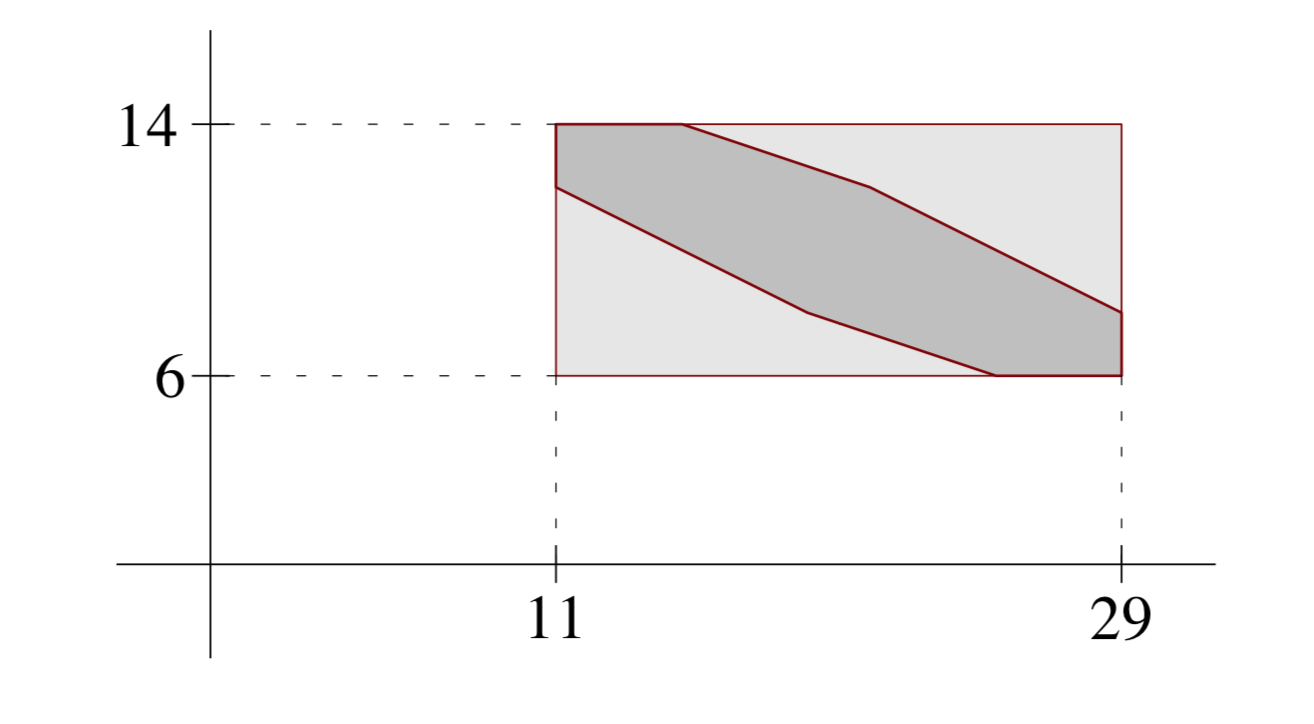
\includegraphics[width=88mm]{fig/IntervalAffineDiff.png}
    \caption{区间算法与仿射算法分析结果对比图} \label{fig:interval_affine_diff}
\end{figure*}

仿射算术并不是在所有情况下都能够比区间算法得到更加准确的结果,如对于非线性运算,特别是由乘除指数开方等构成的复合运算,误差的减小不是绝对的。如区间变量$x \in X = [1,\ 2]$,在计算$f(x) = 1/x$时,利用区间算法的运算规则可以得到其结果为$[1/2 ,\ 1]$,然而使用仿射算术,我们首先需要将$x$改写成仿射形式$\hat{x} = 1.5 + 0.5\varepsilon_1$,然后再使用倒数运算的仿射公式,求得其结果区间为$[0.4142,\ 1]$。

由此可见,由于仿射算法在处理非线性运算时会引入新的误差,所得的界限不一定比区间算法的运算结果紧凑.故在计算函数界限时,需要针对不同函数选取不同算法以期尽快获得尽量紧凑的函数界限.

基于区间算法以及仿射算法,许多静态分析方法被提出以研究数值计算程序中浮点数计算的误差积累情况。Putot\cite{10.1007/978-3-540-24738-8_18}提出了一种针对C代码静态分析技术,其研究了在C程序中每一步计算过程中浮点计算的误差积累情况,通过区间分析的方法,将计算过程中每一步的误差以一个区间的形式表示,对程序进行抽象释义\cite{cousot1977abstract},能够发现程序中引起严重的精度损失的计算操作,也能够验证程序最终的执行结果在一定的误差范围之内。后续Goubault\cite{10.1007/3-540-47764-0_14}使用仿射算法改进了这一静态分析方法,使得该分析方法能够应对一些更加复杂的数值程序,例如解非线性方程的牛顿法\cite{atkinson2008introduction}、共轭梯度法\cite{straeter1971extension}等的数值程序,同时也极大的提升了分析结果的准确性。


\section{符号执行技术}

\subsection{符号执行具体原理}

符号执行是一种广泛用于程序分析、软件安全和软件测试的技术,该技术 在20世纪70年代就被提出,从提出至今已经取得了长足的发展。符号执行可以帮助人们完成高覆盖率的测试用例生成以及发现并定位一些复杂软件系统中非常隐蔽的缺陷。在软件测试领域,符号执行的主要目标是能够高效的探索尽可能多的不同的程序执行路径。对于每一条执行路径,符号执行可以通过约束求解的方式生成触发该执行路径的具体输入,另外还可以检测该执行路径上是否有程序缺陷,包括内存溢出、未捕获的异常等等。从软件测试的角度来看,符号执行可以帮助我们生成高覆盖率的测试用例,从缺陷检测的角度来看,符号执行可以提供能够除法特定缺陷的具体输入,以帮助程序员调试代码,修正缺陷。

符号执行的核心思想是使用符号化的变量而非具体的程序输入去执行程序,程序中所有的中间变量都由符号化的输入变量的表达式来表示,程序最终的输出也不是一个具体的数值,而是一个以符号化的输入变量为参数的一个函数。除了将程序中的输入替换为符号化输入以外,对于每一条程序执行路径,符号执行还需要维护该路径对应的符号执行状态$\sigma$以及路径约束$PC$,其中符号执行状态$\sigma$是一张程序变量与其对应的符号化表达式的对应关系表,而路径约束$PC$通常有一组符号化表达式的交集构成,代表了执行该条路径时程序输入所需要满足的条件。符号执行状态$\sigma$以及路径约束在符号执行过程中都会不断地进行更新,在符号执行结束后,我们可以调用底层约束求解器对路径约束进行求解,求解得到的结果作为程序的具体输入值则可以触发该条执行路径。符号执行会尝试遍历程序的所有路径, 而符号执行过程中的所有程序路径可以通过一棵符号执行树进行表示。

通过以上描述,我们可以总结出符号执行不同于具体执行的几个主要特征:
\begin{itemize}
    \item 符号执行使用符号化的输入代替具体值输入,并将程序中所有变量都使用符号化输入构成的表达式进行表示。
    \item 符号执行为每一条执行路径维护了一个执行状态表$\sigma$以及路径约束$PC$,在符号执行结束时调用约束求解器求解约束得到能够触发该执行路径的程序具体输入。
    \item 程序往往具有多条执行路径,而具体输入一次只能触发其中一条执行路径,而符号执行中程序的所有执行路径构成了一个符号执行树,通过对符 号执行树的所有路径进行遍历,即可完成对程序所有执行路径的遍历。
\end{itemize}

为了更加进一步的说明符号执行于具体执行的区别,我们以图\ref{lst:symexeccode}所示的示例程序来介绍具体执行以及符号执行的不同的执行过程。
\begin{figure}[thbp]
    \begin{lstlisting}[%
      xleftmargin=10em,numberblanklines=true,boxpos=b,%,extendedchars=\true, %inputencoding=utf8%/latin1
      morekeywords={sym_input, ERROR}%keywords={main}
    ]
    int triple(int v) {
        return 3*v;
    }

    void sym_example(int x, int y) {
        z = triple(y);
        if (z == x) {
            if (x > y + 5) {
                ERROR;
            }
        }
    }

    int main() {
        x = sym_input();
        y = sym_input();
        sym_example(x, y);
        return 0;
    }
    \end{lstlisting}
    %\vspace*{-4mm}
    \caption{符号执行示例程序代码片段}
    \label{lst:symexeccode}
    %\vspace*{-4mm}
\end{figure}

在具体执行时,我们假设程序的具体输入是$\{x=3,y=1\}$,程序的具体执行过程如下:执行语句6,其会调用函数triple,返回结果是3,因此,变量$z$被赋值为3;然后顺序执行语句7,是一个if语句,此时$z$与$x$的具体值均为3,满足$z==x$,因此进入该分支;执行语句8,依然为if语句,不满足条件$x>y+5$,程序具体执行结束。由此可见,具体执行只执行了函数sym\_example多条执行路径中的一条。

在符号执行时,首先会创建一个执行状态$\sigma$以及路径约束$PC$,在一开始的时候$\sigma$是一个空集,$PC$为$true$。每当遇到一个语句$var = sym_input()$时,符号执行会将一个新的符号与变量之间的对应关系$var \mapsto s$添加到a中去,这里的$s$是一个新的符号化的变量。在这个例子中,程序的第15-16行会使得原本为空的$\sigma$更新为$\sigma = \{x \mapsto x_0, y \mapsto y_0\}$;每当遇到一个赋值语句$v = e$时,符号执行会将执行状态$\sigma$中的$v$的表达式更新为$\sigma(e)$,也就是使用当前执行状态中的对应关系计算$e$得到的结果。在这个例子中,当我们执行完语句6时,程序的执行状态会被更新成为$\sigma = \{x \mapsto x_0, y \mapsto y_0, z \mapsto 3x_0\}$;每当遇到一个条件分支语句 \texttt{if (}$e$\texttt{) S1 else S2}时,$PC$会被更新成为$PC\wedge\sigma(e)$,对应then分支,同时也会产生一条新的执行路径,其路径约束为$PC'=PC\wedge\neg\sigma(e)$,对应了else分支,这里便不同于具体执行,因为具体执行仅仅会执行这两条分支中的一条,而在符号执行过程中,每一条执行路径均会被记录下来。在此例中,当我们执行完语句7后,会产生两条不同的执行路径分别对应$x_0 = 3y_0$以及$x_0 \neq 3y_0$,同样的,在执行完语句8后,在$x=3y_0$的分支亦会产生两个新的执行路径,其对应的路径约束分别为$(x_0 = 2y_0) \wedge (x_0 > y_0 + 5)$与$(x_0 = 2y_0) \wedge (x_0 \leq y_0 + 5)$。当符号执行遇到结束语句后,当前的符号执行实例便终止了,然后对调用底层求解器求解路径约束得到路径对应的程序的具体输入,在这个具体的例子中,我们可以求解得到三条路径对应的不同的具体输入分别为$\{x = 0,y = 1\}$,$\{x = 3,y = 1\}$和$\{x = 30, y = 10\}$。最终的符号执行结果如表\ref{tbl:symexamres}所示,其符号执行树如\ref{fig:symexectree}所示;

\begin{table}
    \centering
    \begin{tabular}{ccc}
      \toprule
      \textbf{程序路径} & \textbf{路径约束} & \textbf{测试用例} \\
      \midrule
      路径1 & $3y_0 = x_0 \wedge x_0 > y_0 + 5$ & $x = 30, y = 10 $ \\
      路径2 & $3y_0 = x_0 \wedge x_0 \leq y_0 + 5 $ & $x = 3, y = 1$ \\
      路径3 & $3y_0 \neq x_0$ & $x = 0, y = 1$ \\
      \bottomrule
    \end{tabular}
    \caption{程序sym\_example符号执行生成测试用例表}\label{tbl:symexamres}
\end{table}

\begin{figure*}[h]
    \centering
    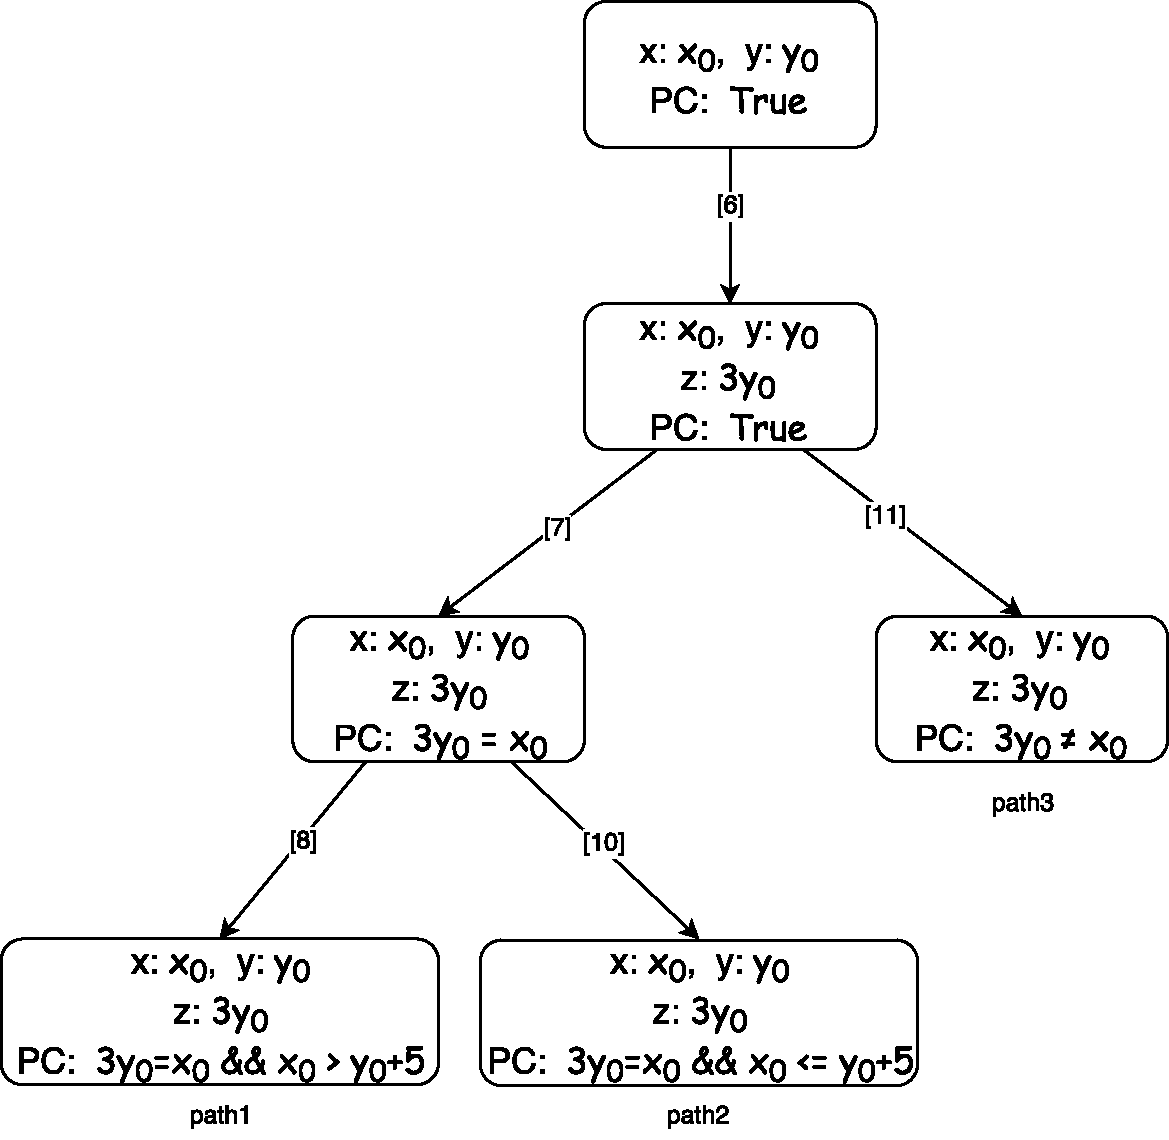
\includegraphics[width=100mm]{fig/SymExecTree.pdf}
    \caption{程序sym\_example符号执行树} \label{fig:symexectree}
 \end{figure*}


在这一小节中,我们简要介绍了符号执行的基本原理以及其具体执行的主要区别。在本文工作中,我们使用符号执行过程对一个数值计算程序的整体的计算过程进行了提取,提取的结果是程序的输出关于程序输入的一个计算式的形式,从上述对符号执行的描述我们可以知道,该计算形式便保存在符号执行状态$\sigma$中,在符号执行结束时,我们可以通过遍历$\sigma$得到其中所有我们关心的变量的计算形式。同时,我们的优化工作是优化对象是一条条的程序路径,在优化完成后,我们要将不同的路径组合在一起形成优化后的程序,所以我们也需要知道每条程序路径对应的约束信息$PC$,这恰恰也是符号执行能够得到的。因此,我们使用符号执行这一技术来完成数值计算程序的计算过程提取的工作。

\section{本章小结}

在这一章节中,我们主要介绍了本问工作的相关背景知识。在第一节中,我们主要介绍了浮点数表示方法以及浮点计算产生误差的原因,浮点数由于无法表示所有的实数因此需要进行舍入操作,由于浮点数的舍入操作会导致浮点数的舍入误差。然后在第二小节中,我们主要介绍了任意精度计算的相关背景知识以及需要使用任意精度计算的原因,在某些情况下浮点精度无法满足计算程序对精度的需求,即便使用扩展的双精度浮点数程序依然存在较大的误差,此时我们便需要使用任意精度类型来完成计算操作。

在第三小节中,我们介绍了两种不同的静态分析方法,分别是基于区间算法的静态分析方法以及基于仿射算法的静态分析方法,阐述了两者的特点以及各自的优缺点。最后我们介绍了符号执行的相关知识,以一个具体的实例简要阐述了符号执行与具体执行的区别并总结了符号执行的特点。

% 第三章方法框架
\chapter{基于随机代数变换的数值程序优化框架}\label{chapter_framework}

\section{优化实例}
在本章中,我们举一个具体的例子来阐释整体的程序优化过程。如图\ref{fig:midarc}所示,在复平面内有两个单位复数$z_1,z_2$,我们需要计算这两个负数在复平面上的角平分线所对应的单位复数$z_3$。显而易见的,由于$z_1,z_2$均为单位复数,计算$z_3$只需要通过以下公式进行计算:

\begin{align}\label{eq:fpex}
    z_3=\frac{z_1+z_2}{\left|z_1+z_2\right|}
\end{align}

软件开发人员根据以上公式,可以非常轻易地实现整个计算过程,代码如图\ref{lst:exoricode}所示。这样的代码非常符合人们的直观感受并且非常易读易维护,然而这样的代码并不是正确并且高效的代码。如果我们使用任意精度类型来实现这样的代码,程序的运行效率会比普通的浮点精度实现慢上成百上千倍。而如果我们使用浮点精度类型来实现这样的代码,后果更为严重,这样的程序甚至是错误的。通过的计算过程的简单分析我们可以知道,当我们使用浮点精度类型去实现这个计算过程时,如果$|z_1+z_2| < \epsilon$的话,其中$\epsilon$是一个很小的正数,整个计算过程将会是不稳定的。

\begin{figure*}[thbp]
   \centering
   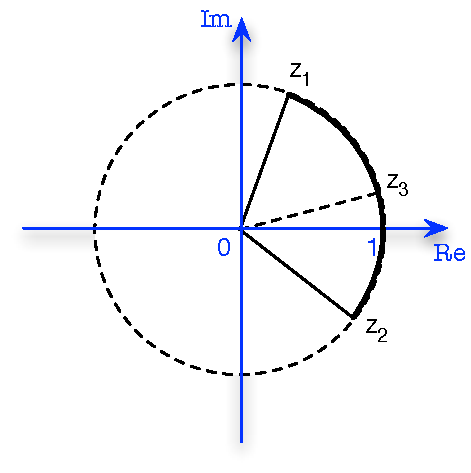
\includegraphics[width=88mm]{fig/ExampleArc_formal.pdf}
   \caption{计算单位复数$z_1,z_2$在复平面内角平分线$z_3$} \label{fig:midarc}
\end{figure*}

当$|z_1+z_2| < \epsilon$时,在程序代码的第4行与第5行,计算$z_1+z_2$时,由于$z_1 \approx -z_2$,这个加法操作会使得计算结果的有效数字位数发生锐减[],导致计算结果的相对误差非常大。而后续第7行的除法操作,由于除数$|z_1+z_2|$是一个非常小的数,会进一步放大前面加法操作的误差,导致程序的计算结果出错。我们实际运行了一下这个程序,在处理器为英特尔酷睿i7 2.9GHz的苹果笔记本MacBook Pro上,以浮点精度类型实现的该计算过程,我们令输入$z_1=e^{i\pi/4},z_2=-z_1*e^{-i \epsilon \pi},\epsilon=10^{-16}$,程序的运行结果$z_3=-0.5547+0.8321i$,显而易见是错误的,其正确结果应该为$z_3=-0.7071+0.7071i$。

\begin{figure}[thbp]
    \begin{lstlisting}[%
      xleftmargin=\columnsep,numberblanklines=true,boxpos=b,%,extendedchars=\true, %inputencoding=utf8%/latin1
      morekeywords={REAL,IComplex}%keywords={main}
    ]
    IComplex midarc(IComplex z1,IComplex z2){
      if(abs(z1)!=1 || abs(z2)!=1)
        throw PreConditionException;
      REAL r = realpart(z1) + realpart(z2);   
      REAL i = imaginary(z1) + imaginary(z2); 
      IComplex sum(r,i);
      IComplex z3 = sum / abs(sum);           
      return z3;
    }
    \end{lstlisting}
    %\vspace*{-4mm}
    \caption{直接使用公式$(z_1+z_2)/|z_1+z_2|$计算$z_3$的任意精度代码}
    \label{lst:exoricode}
    %\vspace*{-4mm}
\end{figure}
    
我们的优化框架可以将图\ref{lst:exoricode}中这样的不稳定的浮点精度的计算过程优化成为稳定高效的浮点精度的计算过程,如图\ref{lst:exoptcode}所示。 原来不稳定的计算过程$z_3=(z_1+z_2)/|z_1+z_2|$被转换成了一种与之在数学上等价的稳定的计算过程,具体来说,$z_1,z_2,z_3$均被表示成了复数的极坐标表示形式,$z_1=e^{i\theta_1},z_2=e^{i\theta_2}$,与此同时,$z_3$的计算过程也被等价的转换成为:

\begin{align}\label{eq:optex}
    z_3=e^{i\frac{\theta_1+\theta_2}{2}}
\end{align}

当$|z_1+z_2|<\epsilon$时,优化后的代码便使用这样稳定的计算过程来计算$z_3$,这样一来,优化后的代码便避免了原本不稳定的计算操作。同样的,我们以输入z$z_1=e^{i\pi/4},z_2=-z_1*e^{-i \epsilon \pi},\epsilon=10^{-16}$来运行优化后的代码,得到的结果即为正确的运行结果$z_3=-0.7071+0.7071i$。

\begin{figure}[thbp]
  \begin{lstlisting}[%
    xleftmargin=\columnsep,numberblanklines=true,boxpos=b,%,extendedchars=\true, %inputencoding=utf8%/latin1
    morekeywords={FComplex}%keywords={main}
  ]
  FComplex midarc(FComplex z1,FComplex z2){
    if((abs(z1)-1)>epsi || (abs(z2)-1)>epsi)
      throw PreConditionException;
    double r = realpart(z1) + realpart(z2);      
    double i = imaginary(z1) + imaginary(z2);    
    FComplex sum(r,i); FComplex z3;              
    if(abs(sum)<epsi){
      double theta1 = atan2(imaginary(z1),realpart(z1));
      double theta2 = atan2(imaginary(z2),realpart(z2));
      double theta3 = (theta1+theta2)/2;
      z3 = FComplex(cos(theta3),sin(theta3));
    }else{
      z3 = sum / abs(sum);                       
    }
    return z3;
  }
  \end{lstlisting}
  %\vspace*{-4mm}
  \caption{优化后的计算$z_3$的浮点精度代码}
  \label{lst:exoptcode}
  %\vspace*{-4mm}
\end{figure}

整个优化过程的主要思想是通过代数式的等价转化,将原本不稳定的浮点精度计算过程替换成为一个与之等价的稳定的计算过程,每次这样的计算过程的替换都必须保证替换前后的计算过程在数学意义上是等价的。这样的替换过程的主要难点在于如何自动地寻找这样一个等价的稳定计算过程,因此本文提出了一种基于随机代数变换的等价表达式搜索算法,将这样一个替换过程转变成为一个搜索的过程。首先,我们会将数值程序的计算过程作为一个整体抽取出来,得到一个计算过程的代数式(在上述例子中,这个代数式便是$z_3=(z_1+z_2)/|z_1+z_2|$),然后我们对该代数式进行随机的代数变换,变换过程以及得到的等价代数式集合如图\ref{fig:eqspace}所示,得到等价代数式集合后,我们会在整个等价集合中随机选取代数式然后继续进行随机的变换,这样迭代下去,一直到我们寻找到一个稳定的计算代数式。当我们找到了稳定的计算代数式后,我们会将这个代数式还原成为可执行代码,并替换原不稳定的计算过程。

\begin{figure}[thb]
  \centering
  \vspace*{1mm}
  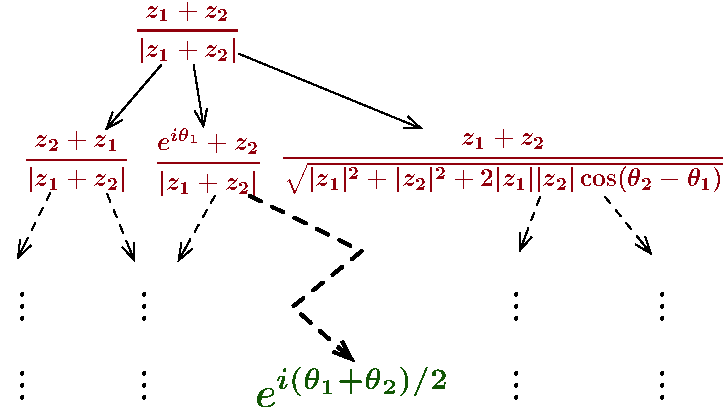
\includegraphics[width=120mm]{fig/EquivalentSpace.pdf}
  \vspace*{1mm}
  \caption{等价代数式变换过程及得到的等价代数式集合} \label{fig:eqspace} %Equivalence Space to Find a Stable Algebraic Form
\end{figure}

\section{方法框架}

在上一小节中我们以一个具体的实例说明了整体的优化过程,在这一小节中,我们将会具体讨论优化框架的具体构成以及一些技术细节。首先,数值程序的优化过程一共分为4个模块,如图\ref{fig:mainframe}所示,包括了稳定性分析模块、计算路径提取模块、随机代数变换模块以及计算路径合并模块。

首先,稳定性分析模块会使用区间分析的技术对原程序进行稳定性的分析,对程序的输入域进行划分,将程序的输入域划分为稳定区间,不稳定区间以及未知区间,这三种不同类型区间的具体含义会在下面具体介绍。紧接着,计算路径提取模块会通过符号执行的方式,将不稳定区间所对应的计算过程进行提取,得到程序输出关于程序输入的一个计算代数形式。然后,随机代数变换模块对上个模块提取到的计算代数式进行数学意义上的等价变换,寻找到原计算过程的等价的稳定的计算形式。最后,路径合并模块将上个模块中的等价稳定计算形式转换成为代码片段,并与原本就稳定的计算路径进行合并,得到最终的优化后程序。

\begin{figure*}[thbp]
  \centering
 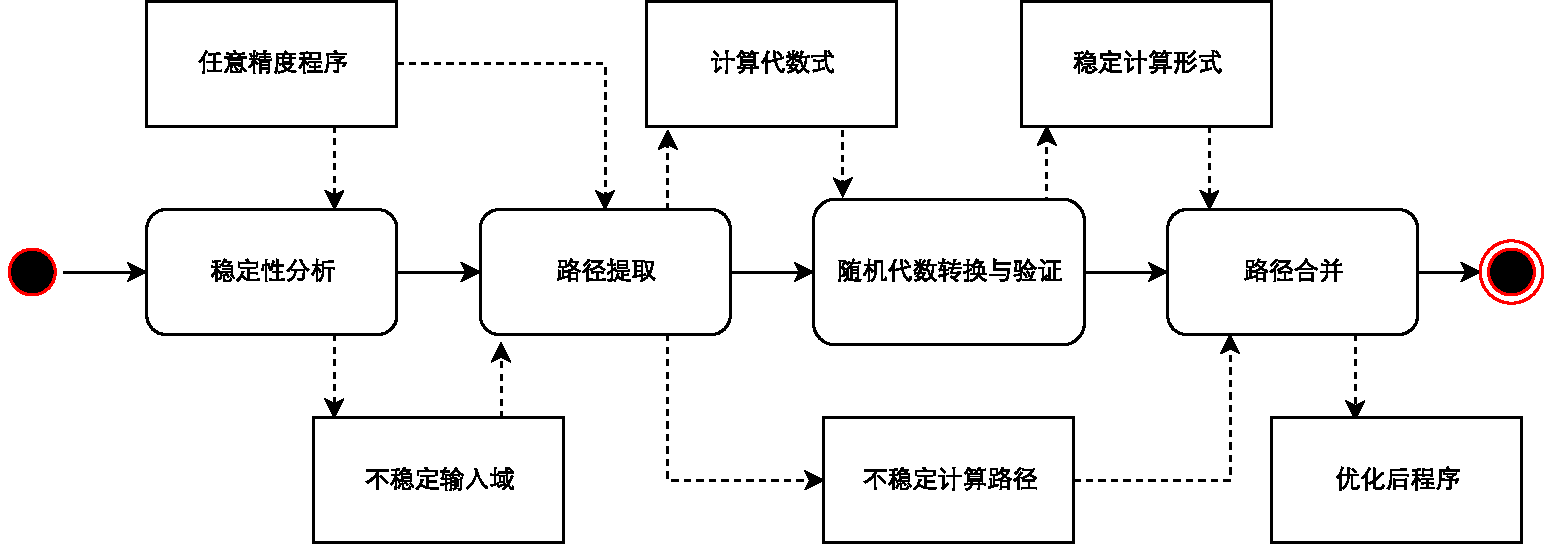
\includegraphics[width=\textwidth]{fig/MainFramework.pdf}
  \caption{数值程序优化框架整体流程图} \label{fig:mainframe}
\end{figure*}

\subsection{稳定性分析}

\subsubsection{稳定输入域定义}
对于一个计算过程$f$来说,我们记其浮点精度实现与任意精度实现所对应的计算过程分别为$F$和$M$,$D$为程序的输入域,对于任意输入$x \in D$,记$F(x)$与$M(x)$分别为以输入$x$去执行计算过程$f$的浮点精度实现以及任意精度实现所得到的计算结果。如果对一个输入域$I \subseteq D$,$I$上的任意输入$x$满足:

\begin{align}
  |\frac{F(x)-M(x)}{M(x)}| < \epsilon
\end{align}

则我们称该输入域$I$为一个稳定的输入域。反之,若存在$x \in $,使得:

\begin{align}
  |\frac{F(x)-M(x)}{M(x)}| \geq \epsilon
\end{align}

则我们称该输入域为不稳定输入域,其中$\epsilon$为参数,是一个很小的正数,用来表示优化框架所能容忍的最大的相对误差。

\subsubsection{输入域划分}

稳定性分析模块会将程序的输入域划分成为稳定输入域以及不稳定输入域,对于稳定输入域部分,由于其本身计算过程已经是稳定的,我们只需要将原计算过程直接使用浮点精度实现即可(对应图\ref{lst:exoptcode}中第13行),然而对于不稳定的输入域,其中包含了会产生误差的输入,优化框架需要对这样的输入域对应的计算过程进行优化(对应图\ref{lst:exoptcode}中第8行到第11行)。

如图\ref{fig:inputspace}为对数值计算程序输入域的一个整体的划分。理论上来讲,整个输入域可以完全的划分成为两个不相交的集合分别为稳定输入域以及不稳定输入域,然而这项工作在现实实践中是非常困难的。通过本节所介绍的分析技术,稳定性分析模块可以识别出部分的稳定输入域以及不稳定输入域,而剩余的无法识别的部分稳定性分析模块会将其归入未知输入域。在整个优化框架中,对于未知输入域以及无法找到稳定计算过程的不稳定输入域,我们会保留原始的任意精度计算过程以保证程序最终计算结果的正确性。

\begin{figure}[tb]
  \centering
  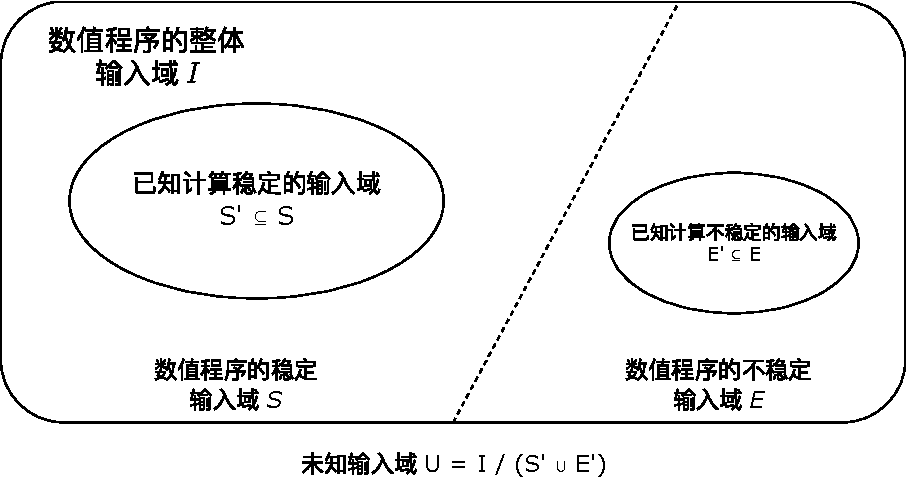
\includegraphics[width=\columnwidth]{fig/InputSpace.pdf}
  \vspace*{1mm}
  \caption{数值计算程序输入域划分图} \label{fig:inputspace} %Equivalence Space to Find a Stable Algebraic Form
\end{figure}

\subsubsection{稳定性分析方法}

稳定分析的整体算法流程如算法\ref{alg:stabilityAnalysis}所示,首先我们会将程序的输入域划分为许多小区间,然后我们对每个小区间的稳定性进行判定,然后再将相同类型的小区间组合起来得到最终的稳定输入域,不稳定输入域以及未知输入域。对于每个小区间,首先,我们会使用区间分析的技术判定该小区间上的最大误差是否在一个可接受的范围内,如果是,我们则认为该小区间是稳定的,将其加入到稳定输入域中。紧接着,如果我们无法判定小区间是稳定的,我们会尝试着去在其中寻找不稳定的输入,我们会在该小区间上随机取一些输入点,将这些输入带入原始任意精度计算过程以及对应的浮点精度计算过程,得到两种计算过程结果的相对误差,若发现有产生较大误差的输入,我们则判定该小区间是不稳定的,否则我们将其纳入未知输入域,因为我们既无法证明该区间是稳定的,又无法找到该区间中的不稳定输入。

\begin{algorithm}[thb]
  \caption{Stablility Analysis Process}
  \label{alg:stabilityAnalysis}
\begin{algorithmic}[1]
\REQUIRE $D$ {{\footnotesize$//$}\small Input Space}
\ENSURE $S', E', U$ {{\footnotesize$//$}\small Stable subspace, Unstable subspace and Unknown subspace}
\STATE $S_d$ $\leftarrow$ split($D$) {{\footnotesize$//$}\small Split input space to a set of small intervals}
\FORALL {$d \in D$}
\IF {$isIntervalStable(d)$}
\STATE add($d$, $S'$)
\ELSE
\STATE $S_p$ $\leftarrow$ randomSamplePoints($d$) {{\footnotesize$//$}\small Randomly sample a few points in $d$}
\FORALL {$p \in S_p$}
\IF{$\neg$ checkStable($p$)}
\STATE add($d$, $E'$)
\ENDIF
\ENDFOR
\STATE add($d$,$U$) {{\footnotesize$//$}\small All sampled points are stable, can't tell whether stable or not}
\ENDIF
\ENDFOR
\end{algorithmic}
\end{algorithm}

\subsection{路径提取}
为了对不稳定输入域上的计算过程进行优化,我们必须将这些计算过程作为一个整体从程序中提取出来,整个计算过程被抽象成为了程序输出关于程序输入的一个计算代数式的形式,这便是路径提取模块所要完成的工作。并且,对于不同输入域上的输入,其对应的计算过程有可能是不同的,对应到程序的控制流图上,即程序在不同输入域上在程序控制流图上所执行的路径时不同的,我们需要对不稳定输入域上涉及到的所有的程序执行路径进行提取。在对程序的执行路径进行提取的同时,路径提取模块同时还会收集每一条执行路径所对应的约束,以便于后续计算过程优化结束后组合程序时使用。原计算过程经过路径提取后被抽象成为了$\{(Constrain, AlgebraForm)\}$这样的二元组的集合的形式,集合中每个元素均为一个二元组,代表了程序控制流图中的一条执行路径,包含了该执行路径的计算代数式以及对应的约束信息。

下面举一个具体的实例来描述路径提取模块的执行结果,如图\ref{lst:symextexam}所示为计算$f(a,b)=|a|+|b|$的数值程序代码片段。显而易见,此程序中总共包括了4条不同的执行路径,优化框架对其进行路径提取的结果如表\ref{tbl:abssumres}所示,不同约束下对应了不同的计算过程。

\begin{figure}[thbp]
    \begin{lstlisting}[%
      numberblanklines=true,boxpos=b,%,extendedchars=\true, %inputencoding=utf8%/latin1
      morekeywords={REAL,IComplex}%keywords={main},
      xleftmargin=.2\textwidth, xrightmargin=.2\textwidth
    ]
    double abs_sum(double a, double b) {
      double r = 0.0;
      if ( a > 0 ) { r += a; } 
      else { r -= a;}
      if ( b > 0 ) { r += b; }
      else {r -= b;}
      return r;
    }
    \end{lstlisting}
    %\vspace*{-4mm}
    \caption{计算$f(a,b)=|a|+|b|$代码片段}
    \label{lst:symextexam}
    %\vspace*{-4mm}
\end{figure}

\begin{table}
  \centering
  \begin{tabular}{ccc}
    \toprule
    \textbf{路径编号} & \textbf{路径约束} & \textbf{计算代数式} \\
    \midrule
    1 & a>0\&\&b>0 & a+b \\
    2 & !(a>0)\&\&b>0 & -a+b \\
    3 & a>0\&\&!(b>0) & a+(-b) \\
    4 & !(a>0)\&\&!(b>0) & (-a)+(-b) \\
    \bottomrule
  \end{tabular}
  \caption{数值计算程序$f(a,b)=|a|+|b|$路径提取结果}\label{tbl:abssumres}
\end{table}

路径提取模块主要使用的符号执行这一技术来完成对计算路径的提取。符号执行是一种广泛用于程序分析、软件安全和软件测试的技术,符号执行于20世纪70年代被提出,至今已经取得了长足的发展。不同于具体的执行,符号执行使用符号化的变量代替程序具体的输入,一步步地执行程序,在执行过程中,所有的中间变量也以符号表达式的形式记录下来。当遇到分支语句时,符号执行会产生新的状态以记录不同的执行分支。

原始的符号执行技术主要用于测试用例生成,当符号执行结束后得到了不同执行路径的约束后,通过将约束交给约束求解器求解可以得到覆盖该执行路径的测试用例。在我们的框架中我们对原始的符号执行技术进行了改进,使其不仅仅记录路径约束,同时也会记录每条执行路径所对应的执行结果。在符号执行过程中,对于程序中每一条执行路径,我们会维护一个符号执行的状态信息$es=(ins, sym, out, c)$,其中$es.ins$表示当前被执行指令,$es.sym$记录了到现在为止的符号执行过程中所收集到的变量以及其对应的符号表达式,$es.out$记录了数值计算程序的所有的输出的变量,最后$es.c$表示执行路劲对应的约束信息。当一个程序执行状态遇到了一条分支指令时,该执行状态也会对应地产生两个新的执行状态$es_1$与$es_2$,分别对应了分支指令的$True$分支与$False$分支。若分支条件为$b$,则$es_1$的路径约束被更新成为$es.c \wedge b$,对应的$es_2$的分支条件则为$es.c \wedge \neg b$。

\begin{algorithm}[thb]
  \caption{Symbolic Trace Extraction Process}
  \label{alg:tractExtract}
\begin{algorithmic}[1]
\REQUIRE $\mathcal{P}, S'$ \hfill {{\footnotesize$//$}\small input program \& stable subspace}
\ENSURE $M_{AF}$ \hfill {{\footnotesize$//$}\small map every output to an algebraic form} %[e_1,\cdots,e_n]
    \STATE $es$ $\leftarrow$ initialSTATE($\mathcal{P}$);
    \FORALL {$i \in$ input($\mathcal{P}$) $\wedge\ i \in \mathbb{F}$}
      \STATE add($es.sym$, $i$); \hfill {{\footnotesize$//$}\small\ declare inputs to be symbols} \label{alg:tractExtract:input}
    \ENDFOR
    \STATE $ES$ $\leftarrow$ \{$es$\}; \hfill {{\footnotesize$//$}\small $ES$ is a state set}
    \WHILE{$\neg$empty($ES$)} \label{alg:tractExtract:iter}
      \STATE $es \leftarrow$ selectSTATE(ES); \label{alg:tractExtract:select}  \hfill {{\footnotesize$//$}\small $es$ is the current state}
      \SWITCH{$es$.$ins$.Type}
      \CASE {fork \hfill {{\footnotesize$//$}\small such as the \texttt{if} statement} \label{alg:tractExtract:fork}}
        \STATE \{$es_1,es_2$\}$\leftarrow$ forkExecution($es$);
        \STATE \textbf{if} {$\exists i \notin S'$, $es_1.c$($i$)} \textbf{then} add(ES, $es_1$);
        \STATE \textbf{if} {$\exists i \notin S'$, $es_2.c$($i$)} \textbf{then} add(ES, $es_2$);
        \STATE remove(ES, $es$);   \label{alg:tractExtract:forkend}
      \ENDCASE
      \CASE {OUTPUT($v$) $\wedge\ v \in \mathbb{F}$ \hfill {{\footnotesize$//$}\small such as \texttt{printf}($v$)}}
        \STATE add($es.out$, $v$); \label{alg:tractExtract:outputv}
      \ENDCASE
      \CASE{$\mathcal{P}$.EXIT} %\hfill {\small$\triangleright$such as \texttt{abort}, \texttt{exit}} \label{alg:main:exit_statement}
        \FORALL {$v \in es.out$}
          \STATE add($M_{AF}$, symtraceAF($v$, $es$)); \label{alg:tractExtract:recordexp} % 我这里没有写, 事实上这一步非常复杂. symtraceAF 会返回一个对应关系 <v, af<v>>, 同时会记录es.c, 真正记录到$M_{AF}$中的是<v, es.c, af<v>>, 如果另一个路径也输出v, 会有不同的es.c
        \ENDFOR
        %\STATE Generate Algebric Forms for V;  \label{alg:tractExtract:v}
        \STATE remove(ES, $es$);
      \ENDCASE
      \DEFAULT
        \STATE symbolicStep($es$); \label{alg:tractExtract:propagationstep}
      \ENDDEFAULT
      \ENDSWITCH  \label{alg:tractExtract:switend}
    \ENDWHILE \label{alg:tractExtract:iterend}
\end{algorithmic}
\end{algorithm}

算法\ref{alg:tractExtract}描述了此模块中使用到的符号执行技术的具体算法流程,首先我们会将所有的输入变量符号化,然后我们便一步步的以符号执行的方式执行程序。当遇到一条分支语句时,便产生不同的不同的执行状态以记录不同的执行分支(第9行至第13行),同时我们的符号执行过程也会收集程序输出所对应的计算表达式(第14、15行),当程序结束时,将所有记录到的程序输出的计算表达式添加到结果集中去(第16行至第20行),剩余的情况则按照正常的符号执行过程来执行。

\subsubsection{循环模型与递归模型}
% TODO

\subsection{随机代数变换}

在路径提取模块中,我们得到了不稳定输入域对应的计算过程对应的代数表达式,在这一个模块中,我们需要寻找能够代替该计算过程的稳定的计算表达式。我们知道,一个计算问题的计算方法是多种多样的,例如经典的求解非线性方程组的解便有牛顿下山法,牛顿迭代法,弦截法等多种不同的计算方式,即便是对于同一种计算方式,使用不同的精度进行实现时其代码的计算稳定性也是不一样的。对于一个复杂的计算程序,数值计算专家需要投入大量的精力去寻找一种稳定的计算方式,来解决该计算问题,并且这样的实现中往往会掺杂许多与计算逻辑无关的精度控制的代码,不仅会耗费专家与程序员们的大量精力,而且会使得程序难以理解,难以维护。举一个具体的实例,glibc科学计算库中的$sin$、$cos$函数的实现总代码行数大概为1000行,而与之对应的,iRRAM任意精度数值计算库中这两个函数的实现总共不到200行,同样的一个函数的实现,由于glibc是通过浮点精度实现,需要对程序的计算误差进行控制,导致了程序总代码量是任意精度实现的5倍。在这一个模块中,我们通过一种计算式随机代数变换的方法,能够自动的将原来非常直接易懂的任意精度代码转换成为高效然而复杂的浮点精度代码。

\subsubsection{随机代数变换算法}

本模块所介绍的这样的自动转换的过程从本质上来讲是一个搜索的过程,我们将数值计算专家所具备的专业领域知识收集成一个规则库的形式,我们应用规则库中的规则对原来不稳定的计算代数式进行等价的变换,然后去寻找稳定的计算形式。具体的搜索过程如算法\ref{alg:stoctrans}所示,对于每一个不稳定的计算代数式,我们会维护一个等价计算代数式集合,在搜索过程的一开始,此集合只包含了上一模块中提取得到的不稳定的计算代数式(算法\ref{alg:stoctrans}第2行),紧接着,我们会在该集合中随机选取一个计算代数式,并在规则库$R_{opt}$中随机选取一条转换规则,并在这个这个计算代数式上运用这条规则得到一个新的与原代数式在数学上等价的计算代数式$e'$(算法\ref{alg:stoctrans}第7行),然后我们需要通过区间分析的技术去验证新产生的计算式$e'$的计算稳定性,若$e'$计算稳定,则$e'$便是我们需要找的稳定的计算过程,否则,我们将$e'$添加到等价计算代数式集合$E_{af}$中去,继续迭代执行整个搜索过程,直到我们找到一个稳定的计算代数式或是搜索超时。值得注意的是,当计算超时时,便意味着优化框架并没有找到等价的稳定的计算过程,此时我们为了保证最终优化后程序的正确性,对于这部分计算过程,我们会保留其原来的任意精度的实现。

\begin{algorithm}[tb]
  \caption{Recursive Algebraic Transformation}
  \label{alg:stoctrans}
\begin{algorithmic}[1]
\REQUIRE $S_{AF}$ \hfill {{\footnotesize$//$}\small set of algebraic forms}
\ENSURE $M_{T}$  {{\footnotesize$//$}\small map every input form to a stable expression} %\hfill [e_1,\cdots,e_n]
    \FORALL {$af \in S_{AF}$}
      \STATE $E_{af}$ $\leftarrow$ \{$af$\}; \hfill {{\footnotesize$//$}\small build an equivalent set for search} \label{alg:stoctrans:eqset}
      \STATE $e_t$ $\leftarrow$ NIL; \hfill {{\footnotesize$//$}\small the target expression for substitution}
      \REPEAT
        \STATE $e$ $\leftarrow$ selectRandom($E_{af}$); \label{alg:stoctrans:expselect}%{{\footnotesize$//$ select an equivalent exp}}
        \STATE $rule$ $\leftarrow$ pickStochasticConform($R_{opt}$, $e$); \label{alg:stoctrans:rulepick}
        \STATE $e'$ $\leftarrow$ transform($e$, $rule$); \label{alg:stoctrans:applytrans}
        \IF{stableVerification($e'$)} \label{alg:stoctrans:stableverify}
          \STATE $e_t$ $\leftarrow$ $e'$ \label{alg:stoctrans:getet}
        \ELSE
          \STATE $E_{af}$.add($e'$); \label{alg:stoctrans:putbackep}%\hfill {{\footnotesize$//$}\small add the transformed expression in }
        \ENDIF
      \UNTIL {$e_t = $ NIL $\wedge$ !TIME\_OUT}
      \STATE $M_{T}$.add($af$, $e_t$); \label{alg:stoctrans:resultmap}
    \ENDFOR
\end{algorithmic}
\end{algorithm}

\subsubsection{转换规则库}

我们的优化框架收集并实现了一系列的转换规则形成了一个转换规则库$R_{opt}$,这些转换规则均是根据数值计算专家所具备的专业知识总结而来并且是可扩展的,当规则库中的规则越来越丰富时,我们工具的优化能力相对应的也会越来越强大。
 
本小节的剩余部分列举了规则库中当前实现的大部分转换规则,每一条转换规则都包含了待匹配形式以及转换后形式,我们会在计算代数式中去匹配待匹配的计算形式,若匹配成功,我们则可以将其转换成为对应的转换后形式,所有的转换规则在数学意义上均为等价的。

\vspace{1mm}
\begin{center}
{\kaishu\zihao{4} 基础操作规则}
\end{center}
\vspace{1mm}

\begin{itemize}
  \item {\kaishu 负号规则} 
  \begin{gather*}
  -A \longleftrightarrow (-1) \times A 
  \end{gather*}

  \item {\kaishu 减法规则} 
  \begin{gather*}
  A - B \longleftrightarrow A + (-B) 
  \end{gather*}

  \item {\kaishu 除法规则} 
  \begin{gather*}
  A / B \longleftrightarrow A \times (1 / B) 
  \end{gather*}

  \item {\kaishu 对数规则} 
  \begin{gather*}
  e^{\ln X} \longleftrightarrow X  
  \end{gather*}
\end{itemize}

\vspace{1mm}
\begin{center}
{\kaishu\zihao{4} 基本代数规则}
\end{center}
\vspace{1mm}

\begin{itemize}
  \item {\kaishu 交换律规则} 
  \begin{gather*}
  A \odot B \longleftrightarrow B \odot A  
  \end{gather*}

  \item {\kaishu 结合律规则} 
  \begin{gather*}
  A \odot B \odot C \longleftrightarrow A \odot (B \odot C) 
  \end{gather*}

  \item {\kaishu 分配率规则} 
  \begin{gather*}
  A \times (B + C) \longleftrightarrow A \times B + A \times C 
  \end{gather*}
\end{itemize}

\vspace{1mm}
\begin{center}
{\kaishu\zihao{4} 分式规则}
\end{center}
\vspace{1mm}

\begin{itemize}
  \item {\kaishu 通分规则} 
  \begin{gather*}
  A / B + C / D \longleftrightarrow (AD+BC) / BD 
  \end{gather*}

  \item {\kaishu 约分规则} 
  \begin{gather*}
  AN / BN \longleftrightarrow A / B 
  \end{gather*}

  \item {\kaishu 分子规则} 
  \begin{gather*}
  (A+B) / (C+D) \longleftrightarrow (A+B)(A-B) / ((C+D)(A-B)) 
  \end{gather*}

  \item {\kaishu 分母规则} 
  \begin{gather*}
  (A+B) / (C+D) \longleftrightarrow (A+B)(C-D) / ((C+D)(C-D)) 
  \end{gather*}
\end{itemize}


\vspace{1mm}
\begin{center}
{\kaishu\zihao{4} 多项式规则}
\end{center}
\vspace{1mm}

\begin{itemize}
  \item {\kaishu 累加规则} 
  \begin{gather*}
  \begin{array}{@{}c@{}} A_1 + A_2 + A_3 + ... + A_n \\ \forall A_{si}, A_{sj} \in \{A_1, A_2, ... , A_n\}, \text{ s.t. } i<j \rightarrow     A_{si}\leq A_{sj} \end{array} \\
  \downarrow \\
  A_{s1} + A_{s2} + A_{s3} + ... + A_{sn}
  \end{gather*}

  % itemize中段首使用两个全角空格来缩进
    在科学计算方法中,我们有避免误差危害的若干原则,其中有一条便是注意运算次序,防止“大数”吃掉“小数”,如有多个数相加减,应按照绝对值有小到大的次序进行运算。针对这条原则,我们设计了这一条累加规则,因为在累加的过程中,如果不注意运算次序,在计算前N项和与第N+1项的加法操作时,由于加法操作的两边数量级相差很大,非常容易出现“大数”吃“小数”的情况,因此我们将这样的计算过程进行等价的转换,先对原计算项按照绝对值大小进行排序,然后再进行累加操作,避免产生误差。\\

  \item {\kaishu 霍纳规则} 
  \begin{gather*}
  A_0 + A_1X + A_2X^2 + A_3X^3 + ... + A_nX^n \\
  \downarrow \\
  A_0 + X(A_1 + X(A_2 + ... + X(A_{n-1} + XA_n)))
  \end{gather*}

    霍纳算法是一种计算一元多次多项式求值的高效算法,由英国数学家威廉·乔治·霍纳发现并证明。其具体的算法如下,对于一个一元多次多项式:

  \begin{gather*}
    p(x) = \sum_{i=1}^{n} a_ix^i = a_0+a_1x+a_2x^2+a_3x^3+...+a_nx^n
  \end{gather*}

  其中$a_0,...,a_n$为实数,给定一个$x$的值$x_0$,我们需要计算$p(x0)$。为了完成这样的计算,我们首先定义一系列常数:

  \begin{equation*}
    \begin{split}
    b_n & := a_n \\
    b_{n-1} & := a_{n-1} + b_nx_0 \\
    & \vdots  \\
    b_0 & := a_0 + b_1x_0
    \end{split}
  \end{equation*}

  则$b_0$便是我们需要计算的多项式的值。证明过程如下,我们可以将$p(x)$写成如下的形式:

  \begin{gather*}
    p(x) = a_0+x(a_1+x(a_2+...+x(a_{n-1}+a_nx))) 
  \end{gather*}

  不断将$b_i = a_i + b_{i+1}x_0$带入可以得到:

  \begin{equation*}
    \begin{split}
    p(x_0) & = a_0+x_0(a_1+x_0(a_2+...+x_0(a_{n-1}+a_nx_0))) \\
           & = a_0+x_0(a_1+x_0(a_2+...+x_0(b_{n-1}))) \\
           & \vdots \\
           & = a_0 + x_0b_1 \\
           & = b_0
    \end{split}
  \end{equation*}

    因此,最终算出的$b_0$的值即为多项式求值的结果。通过霍纳形式计算一元多次多项式的值可以显著提高计算效率,对于一个$n$次的多项式函数,用常规方法(用重复乘法计算幂,再把各项相加)计算出结果最多需要$n$次加法和$\frac{(n^{2}+n)}{2}$次乘法。若用迭代的方法计算幂则需要$n$次加法和$2n+1$次乘法。如果计算中的数值数据是以字节方式储存的,那么常规方法约需要$x$占用的字节的$2n$倍空间。而使用霍纳算法时,至多只需作$n$次加法和$n$次乘法,最多需要x占用的字节的n倍空间。因此,我们通过设计这样一条基于霍纳算法的转换规则来提高数值计算程序中一元多次多项式的计算效率。\\

  \item {\kaishu 偏移规则} 
  \begin{gather*}
  A_0 + A_1X + A_2X^2 + A_3X^3 + ... + A_nX^n \\
  \downarrow \\
  B_0 + B_1(X - m) + B_2(X - m)^2 + ... + B_n(X - m)^n \text{ where } B_i=\sum_{k=0}^{n-i} \binom{i+k}{i}A_{i+k}m^k
  \end{gather*}
\end{itemize}

\vspace{1mm}
\begin{center}
{\kaishu\zihao{4} 三角函数规则}
\end{center}
\vspace{1mm}

\begin{itemize}
  \item {\kaishu Tan规则} 
  \begin{gather*}
  \tan X \longleftrightarrow \sin X / \cos X
  \end{gather*}

  \item {\kaishu Sec规则} 
  \begin{gather*}
  \tan X \longleftrightarrow 1 / \cos X
  \end{gather*}

  \item {\kaishu Cot规则} 
  \begin{gather*}
  \cot X \longleftrightarrow \cos X / \sin X
  \end{gather*}

  \item {\kaishu Csc规则} 
  \begin{gather*}
  \csc X \longleftrightarrow 1 / \sin X
  \end{gather*}

  \item {\kaishu Sin加法规则} 
  \begin{gather*}
  \sin(A+B)  \longleftrightarrow \sin A \cos B + \cos A \sin B
  \end{gather*}
  
  \item {\kaishu Cos加法规则} 
  \begin{gather*}
  \cos(A+B)  \longleftrightarrow \cos A \cos B - \sin A \sin B
  \end{gather*}
\end{itemize}

\vspace{1mm}
\begin{center}
{\kaishu\zihao{4} 泰勒公式规则}
\end{center}
\vspace{1mm}

\begin{itemize}

  \item {\kaishu e的泰勒展开规则} 
  \begin{gather*}
  1 + X + X^2 / 2! + X^3 / 3! + X^4 / 4! + ... \longleftrightarrow \exp(X)
  \end{gather*}

  \item {\kaishu 对数函数泰勒展开规则} 
  \begin{gather*}
  - X - X^2 / 2 - X^3 / 3 - ... \wedge\ \left|X\right| < 1 \longleftrightarrow  \ln(1-X)
  \end{gather*}

  \item {\kaishu Sin函数泰勒展开规则} 
  \begin{gather*}
  X - X^3/3! + X^5/5! - X^7/7! + ... \longleftrightarrow  \sin(X)
  \end{gather*}

  \item {\kaishu Cos函数泰勒展开规则} 
  \begin{gather*}
  1 - X^2/2! + X^4/4! - X^6/6! + ... \longleftrightarrow  \cos(X)
  \end{gather*}

    在数学上,泰勒级数是指将一个函数表示成为无限项多项式求和的形式,也就是级数的形式,这些相加的项均为函数在某一点的求导所得。泰勒级数由英国数学家布鲁克·泰勒于1715年发表并命名。在实际运用中,因为不可能进行无限项的加法,泰勒级数需要截断,只取有限项进行加法,一个函数的有限项泰勒级数叫作泰勒多项式。在科学计算领域常用泰勒多项式来估算一个函数的值,由于只取了泰勒级数中的有限项,这种估算是存在误差的,可以使用泰勒定理来估算这种误差,保证程序的可靠性。

    泰勒级数的定义,一个在实数或复数$a$邻域上的无穷可微实变函数或复变函数$f(x)$的泰勒级数是如下的幂级数:

  \begin{gather*}
    f(a)+\frac{f'(a)}{1!}(x-a)+\frac{f''(a)}{2!}(x-a)^2+\frac{f'''(a)}{3!}(x-a)^3+...
  \end{gather*}

  这里,$n!$表示$n$的阶乘,而 ${f^{(n)}(a)}$表示函数$f$在点$a$处的$n$阶导数。


    在规则库中,我们添加了几个非常常用的函数的泰勒展开式规则,包括指数函数,对数函数,Sin函数的泰勒多项式的形式,尝试使用泰勒多项式对该函数进行计算,亦或者是当我们发现该计算过程是在使用泰勒多项式计算某个函数值时,我们将其替换为C库中的函数实现,以提成程序的执行效率以及精度。

\end{itemize}

\vspace{1mm}
\begin{center}
{\kaishu\zihao{4} 复数规则}
\end{center}
\vspace{1mm}

\begin{itemize}

  \item {\kaishu 复数的极坐标表示形式规则} 
  \begin{gather*}
    A + Bi \longleftrightarrow \sqrt {A^2 + B^2} e^{i\arctan(B/A)}
  \end{gather*}
  
    复数有多种不同的表示形式,包括直角坐标形式(也叫作笛卡尔坐标形式),极坐标形式。

    复数的基本单位是$i=\sqrt{-1}$,复数空间中的每个数都可以表示为$a+bi$的形式,其中$a$被称为实部,$b$被称为虚部,这种表示方法被称为复数的直角坐标形式。对应到复平面上,复平面的横纵坐标分别表示了复数的实部和虚部。

    复数同样也可以通过极坐标的形式表示,每个复数$z$由其模$r = |z|$ ,以及其幅角$\phi=\arg(z)$唯一表示。其中$r=0$时,任意值的$\phi$均表示同一个复数,此时通常会将$\arg(0)$设置为$0$。当$r>0$时,幅角模以$2\pi$后时唯一的,也就是说,如果复数辐角的两个值只相差精确的$2\pi$的整数倍数,则它们被认为是等价的,通常情况下,我们会将$\phi$限制在$(-\pi, \pi]$内。于是我们就得到了复数的极坐标表示形式$z =(r, \phi)$。

    极坐标不同表示之间可以相互转换,复数的极坐标形式到直角坐标形式的转换关系为:

  \begin{equation*}
    \begin{split}
      x &= r \cos \phi \\
      y &= r \sin \phi
    \end{split}
  \end{equation*}

  复数的直角坐标形式到极坐标形式的转换关系为:

  \begin{equation*}
    \begin{split}
      r & = \sqrt{x^2+y^2} \\
      \phi & = 
      \begin{cases}
        \arctan(\frac{y}{x}) & \quad \text{if } x > 0 \\
        \arctan(\frac{y}{x}) + \pi & \quad \text{if } x < 0 \text{ and } y \geq 0 \\
        \arctan(\frac{y}{x}) - \pi & \quad \text{if } x < 0 \text{ and } y < 0 \\
        +\frac{\pi}{2} & \quad \text{if } x = 0 \text{ and } y > 0 \\
        -\frac{\pi}{2} & \quad \text{if } x = 0 \text{ and } y < 0 \\
        \text{undefined} & \quad \text{if } x = 0 \text{ and } y = 0 \\
      \end{cases}  
    \end{split}
  \end{equation*}

  前面的公式要求非常繁杂的情况区分。但是很多编程语言提供了经常叫做atan2一个变体的反正切函数来处理这些细节。\\

  复数的极坐标形式还可以通过欧拉公式写成如下的形式:

  \begin{equation*}
    z = r e^{i\phi}
  \end{equation*}

  复数在极坐标形式下,其乘除法、指数和开放根要比直角坐标形式下简单许多,例如复数的乘除法操作:

  \begin{gather*}
    r_1 e^{i\phi_1} \cdot r_2 e^{\phi_2} = r_1r_2 e^{i(\phi_1+\phi_2)} \\
    \frac{r_1 e^{i\phi_1}}{r_2 e^{\phi_2}} = \frac{r_1}{r_2}e^{i(\phi_1-\phi_2)}
  \end{gather*}

  因此我们设计了一条关于复数不同表示形式的转换规则,可以提高关于复数的数值计算程序的运行效率。

\end{itemize}

\vspace{1mm}
\begin{center}
{\kaishu\zihao{4} 伽玛函数规则}
\end{center}
\vspace{1mm}

\begin{itemize}

  \item {\kaishu 斯特林伽玛规则} 
  \begin{gather*}
  (X-0.5)\ln X-X+\ln {2\pi}/2+\sum _{n=1}^{N}{{B_{2n}}/(2n(2n-1)X^{2n-1})} \\
  \downarrow \\
  \ln \Gamma(X)
  \end{gather*}

  \item {\kaishu 伽玛函数定义规则} 
  \begin{gather*}
    \Gamma(X) \longleftrightarrow X\Gamma(X-1) 
  \end{gather*}

  \item {\kaishu 伽玛函数近似规则} 
  \begin{gather*}
  \Gamma(X)\ \wedge\ \left|X\right| < \varepsilon \longleftrightarrow 1/X - \gamma \\
  \Gamma(X)\ \wedge\ \left|X+1\right| < \varepsilon \longleftrightarrow \gamma - 1 - 1/(X + 1) \\
  \Gamma(X)\ \wedge\ \left|X+2\right| < \varepsilon \longleftrightarrow (8 - 4 \gamma + 3 X - 2 \gamma X)/(4X + 8)
  \end{gather*}

  伽玛函数是阶乘函数在实数和复数上的扩展,对于实数部分为正的复数z,伽玛函数定义为:

  \begin{equation*}
    \Gamma (x) = \int_{0}^{\infty} \frac{t^{z-1}}{e^t} \mathrm{d}t 
  \end{equation*}

  此定义可以用解析开拓原理拓展到整个复数域上,非正整数外。特别的,当$n$为正整数时,伽玛定义为:

  \begin{equation*}
    \Gamma (n) = (n-1)!
  \end{equation*}

  伽玛斯特林规则实际上是使用斯特林公式对伽玛函数的一种近似计算。斯特林公式是一条用来去$n$的阶乘近似值的数学公式,其公式如下:

  \begin{equation*}
    n! \approx \sqrt{2\pi n}(\frac{n}{e})^n
  \end{equation*}

  对于所有的正整数$n$,有:

  \begin{equation*}
    n! = \prod (n) = \Gamma (n+1)
  \end{equation*}

  然而,伽玛函数与阶乘函数不同,其在实数与复数上也有定义,尽管如此,斯特林公式仍然是适用的,因此我们可以得到:
  
  \begin{equation*}
    \ln \Gamma(z) = (z-\frac{1}{2})\ln z - z + \frac{\ln 2 \pi}{2} + 2 \int_{0}^{\infty}\frac{\arctan \frac{t}{z}}{\exp{2\pi t}-1} \mathrm{d} t
  \end{equation*}

  对上述式子反复进行分部积分,我们可以得到以下渐进展开式:

  \begin{equation*}
    \ln \Gamma(z) = (z-\frac{1}{2})\ln z - z + \frac{\ln 2 \pi}{2} + \sum_{n=1}^{\infty}\frac{(-1)^{n-1}B_n}{2n(2n-1)z^{2n-1}}
  \end{equation*}

  其中$B_n$是第$n$个伯努利数,以上便是斯特林伽玛规则的由来,利用斯特林公式对伽玛函数近似计算以提高程序的执行效率。

  伽玛函数近似规则是通过一定的数学推导得到的伽玛函数在特定点附近的近似计算方式,相比于使用斯特林公式来近似计算,近似规则中的这些计算具有精度更高,运行速度更快的特点。

\end{itemize}




\subsection{路径合并}



% 第四章实验与实现
\chapter{实验与工具实现}\label{chapter_experiment}

\section{工具}

在上一章的方法中我们介绍了整体的优化框架一共分为4个不同的模块,分别是稳定性分析模块、计算路径提取模块、随机代数变换模块以及路径合并模块,在我们工具的实现中,每个模块都有对应的具体实现,其中路径提取模块以及随机代数变换模块存在一些技术难点,下面做具体介绍。

\subsection{基于KLEE符号执行的计算路径提取模块}

在这一模块中,我们通过符号执行的方式,将程序不稳定输入域上的计算路径提取出来。这一工作主要是基于符号执行技术来完成的,完全由自己手工来设计并实现一个符号执行工具将会是一项浩大的工程,因此我们选择对现有的符号执行工具进行改动,在其上添加新的功能以完成路径提取的工作。在这里我们选择KLEE作为我们的目标工具,KLEE本身是由斯坦福大学开发并发布的一个符号执行工具,其主要特点是能够通过符号执行的技术对复杂代码或者系统产生高覆盖率的测试用例。KLEE使用符号化的输入代替所有可能的具体的输入值,程序执行过程中的所有变量均会被表示成为关于这些符号化输入的表达式,并在遇到分支语句时构成对应路径的分支约束。从以上过程可以发现,KLEE能够完整的提供包括输入变量符号化,路径约束生产,符号执行等功能,因此我们选择在KLEE的基础上实现计算路径提取的功能。

然而,KLEE本身的功能并不完善,我们需要对KLEE进行改进以得到我们所需要的结果。我们主要对KLEE进行了以下改动,首先添加了对输出变量的识别功能,我们会在原数值计算程序中对需要输出的变量做类似于插桩的操作,将其标记为输出变量,表示我们需要在提取此变量关于程序输入的一个计算表达式,在KLEE的符号执行时,一旦遇到这样的变量,KLEE需要能够识别之,并在符号执行结束后在输出模块中将此变量对应的计算表达式输出。此外,我们的进行路径提取所得到的计算表达式中是必须能够包含一些基础的数学库函数的(比如sin、cos、ln函数等),然而KLEE在符号执行时却跳转入这些函数内部继续进行符号执行,这是我们不想看到的,为此,我们使KLEE在符号执行时有意的去忽略这些数学库函数,将其直接作为一个函数记录下来,而不是去做进一步的符号执行。最后是计算表达式的输出模块,在符号执行完成时,KLEE需要能够将需要的输出变量的计算表达式输出。

路径提取的结果最终会保存在一个路径文件中,对于如图\ref{lst:e_example_code}所示的使用泰勒级数近似计算自然对数e的数值计算程序,其对应抽取得到路径文件如图\ref{lst:e_example_pathfile}所示,路径文件中各个属性想详细解释见表\ref{tab:pathfile_attributes}。


\begin{figure}[thbp]
    \begin{lstlisting}[%
      xleftmargin=\columnsep,numberblanklines=true,boxpos=b,%,extendedchars=\true, %inputencoding=utf8%/latin1
      morekeywords={REAL, INTEGER}%keywords={main}
    ]
                REAL e_approx(INTEGER n) {
                    REAL z = 2; 
                    REAL y = 1;
                    for (INTEGER i = 0; i < n; ++i) {
                        y = y / i;
                        z = z + y;
                    }
                    return z;
                }
    
    \end{lstlisting}
    %\vspace*{-4mm}
    \caption{泰勒级数近似计算自然对数$e$程序代码}
    \label{lst:e_example_code}
    %\vspace*{-4mm}
\end{figure}


\begin{figure}[thbp]
\begin{lstlisting}[language=json,firstnumber=1]
{
    "program_name": "e_example",
    "function_name" : "e_approx",
    "variables" : {"n": "integer", "z": "decimal"},
    "input_variables": ["n"],
    "return": "z",
    "paths": [{
        "constrain": "true", 
        "path": ["procedure:p", "loop:l"]}],
    "loops": {
            "l": {
                "variables": {"i": "integer", "y": "decimal"},
                "initialize": {"i": "1", "y": "1.0"},
                "loop_body":[{
                    "constrain": "i<n",
                    "path": ["procedure:pp"],
                    "break": "false"
                    },
                    {
                    "constrain": "!(i<n)",
                    "path":[],
                    "break": "true"
                    }]
        }
    },
    "procedures": {
        "p": [["z", "1"]],
        "pp": [["y", "y/i"], ["z", "z+y"], ["i", "i+1"]]
    }
}
\end{lstlisting}
\caption{泰勒级数近似计算自然对数$e$程序路径文件}
\label{lst:e_example_pathfile}
\end{figure}

\newcommand{\tabincell}[2]{
    \begin{tabular}{@{}#1@{}}#2\end{tabular}
} 
\begin{table}[!t]  
    \centering  
    \scriptsize  
    \begin{tabular}{ll}  
      \\[-2mm]  
      \hline  
      \hline\\[-2mm]  
      {\bf \small 属性}  &   {\bf\small 含义}\\  
      \hline  
      \vspace{1mm}\\[-3mm]  
      program\_name     &   \tabincell{l}{程序名称}\\  
      \vspace{1mm}  
      function\_name    &   \tabincell{l}{函数名称}\\  
      \vspace{1mm}  
      variables         &   \tabincell{l}{所涉及到的变量及其对应类型}\\  
      \vspace{1mm}  
      intput\_variables &   \tabincell{l}{程序的输入变量}\\  
      \vspace{1mm}  
      output\_variables &   \tabincell{l}{程序的输出变量}\\  
      \vspace{1mm}  
      paths             &   \tabincell{l}{路径提取所得到的计算路径,为一个列表结构,列表中每个元素均为\\一个(约束,计算路径)二元组}\\  
      constrain         &   \tabincell{l}{计算路径对应的约束信息}\\  
      \vspace{1mm}  
      path              &   \tabincell{l}{一条计算路径,被抽象成为一个以procedure或是loop结构的列表的\\形式}\\  
      \vspace{1mm}  
      loops             &   \tabincell{l}{程序中涉及到的所有的循环信息}\\  
      \vspace{1mm}  
      loop\_body        &   \tabincell{l}{循环体信息,同样以计算路径的方式来表示,为一个列表结构,每个元\\素除了约束以及计算路径外,还附带了是否为循环出口的标记}\\  
      \vspace{1mm}  
      break             &   \tabincell{l}{循环体中的路径用来标记该路径是否为循环出口的标志}\\  
      \vspace{1mm}  
      procedures        &   \tabincell{l}{程序中所涉及到的所有的过程语句的信息,可以理解为顺序执行的一段\\代码,以列表形式给出,每个元素包含了变量及其对应计算形式信息}\\  
      \hline  
      \hline  
    \end{tabular}  
    \caption{路径文件属性说明}  
    \label{tab:pathfile_attributes}  
\end{table} 


\subsection{基于规则模板的随机代数变换引擎}

在前面的章节我们介绍了一个基于规则库的随机代数变换方法,来寻找一个不稳定计算过程的等价稳定计算形式。随机代数变换的核心是转换规则库,为了能够方便我们灵活的添加与删除规则,我们实现了一个随机代数变换引擎,规则库以模板文件的形式给出,我们可以非常容易地在规则库中添加新的规则。该随机代数变换引擎主要使用到了ANTLR(Another Tool for Language Recognition)库,该库是一个语法解析器的生成器,我们首先需要定义模板文件的语法,ANTLR可以自动地帮助我们生成该语法对应的解析器。该解析器解析规则模板文件能够得到每一条规则对应的语法树结构,在整个语法树结构上,我们去完成原始表达式形式的匹配,如果匹配成功,我们则将原始表达式转换成为对应的转换后的计算形式。

模板文件每一条规则的语法如下所示:

 \begin{gather*}
    \text{rule\_name} : \text{origin\_expr} \rightarrow \text{transformed\_expr} @ \text{constrain}
 \end{gather*}

 其中rule\_name表示规则名称,origin\_expr表示转换前的计算表达式,也就是需要我们进行匹配的计算表达式,transfromed\_expr表示转换后的计算表达式,constrain表示进行这样的转换需要满足的约束。表格\ref{tab:rule_list}列举了工具当前版本的模板文件中所实现的转换规则,如果我们后续需要添加新的转换规则,只需要在模板文件中添加即可。

\begin{table}[!t]  
    \centering  
    \scriptsize  
    \begin{tabular}{lc}  
      \\[-2mm]  
      \hline  
      \hline\\[-2mm]  
      {\bf \small Rule Name}  &   {\bf\small Content}\\  
      \hline  
      \vspace{1mm}\\[-3mm]  
      Negative     &   \tabincell{l}{$-A \leftrightarrow (-1) * A$}\\  
      \vspace{1mm}  
      Minus    &   \tabincell{l}{$A - B \leftrightarrow A + (-B)$}\\  
      \vspace{1mm}  
      Divide &   \tabincell{l}{$A / B \leftrightarrow A*(1/B)$}\\  
      \vspace{1mm}  
      CommutationPlus &   \tabincell{l}{$A + B \leftrightarrow B + A$}\\  
      \vspace{1mm}  
      CommutationMultiply &   \tabincell{l}{$A * B \leftrightarrow B * A$}\\  
      \vspace{1mm}  
      AssociationPlus &   \tabincell{l}{$A + B + C \leftrightarrow A + (B + C)$}\\  
      \vspace{1mm}  
      AssociationMultiply &   \tabincell{l}{$A * B * C \leftrightarrow A * (B * C)$}\\  
      \vspace{1mm}  
      Distribution1 &   \tabincell{l}{$A * (B + C) \leftrightarrow A * B + A * C$}\\  
      \vspace{1mm}  
      Distribution2 &   \tabincell{l}{$(A + B) * C) \leftrightarrow A * C + B * C$}\\  
      \vspace{1mm}  
      Distribution3 &   \tabincell{l}{$(A + B) / C) \leftrightarrow A / C + B / C$}\\  
      \vspace{1mm}  
      CommDenominator &   \tabincell{l}{$A/B+C/D \leftrightarrow (A*D+B*C)/(B*D)$}\\  
      \vspace{1mm}  
      FracReduction &   \tabincell{l}{$(A*N)/(B*N) \leftrightarrow A/(B)$}\\  
      \vspace{1mm}  
      NumeratorForm &   \tabincell{l}{$(A+B)/(C+D) \leftrightarrow (A+B)*(A-B)/((C+D)*(A-B))$}\\  
      \vspace{1mm}  
      DenominatorForm &   \tabincell{l}{$(A+B)/(C+D) \leftrightarrow (A+B)*(C-D)/((C+D)*(C-D))$}\\  
      \vspace{1mm}  
      Tan &   \tabincell{l}{$\tan(x) \leftrightarrow \sin(x)/\cos(x)$}\\  
      \vspace{1mm}  
      Sec &   \tabincell{l}{$\sec(x) \leftrightarrow 1/\cos(x)$}\\  
      \vspace{1mm}  
      Csc &   \tabincell{l}{$\csc(x) \leftrightarrow 1/\sin(x)$}\\  
      \vspace{1mm}  
      Cot &   \tabincell{l}{$\cot(x) \leftrightarrow \cos(x)/\sin(x)$}\\  
      \vspace{1mm}  
      SinPlus &   \tabincell{l}{$\sin(A+B) \leftrightarrow \sin(A)*cos(B)+cos(A)*\sin(B)$}\\  
      \vspace{1mm}  
      CosPlus &   \tabincell{l}{$\cos(A+B) \leftrightarrow \cos(A)*\cos(B)-\sin(A)*\sin(B)$}\\  
      \vspace{1mm}  
      TayporExp &   \tabincell{l}{$\text{sum}(k, 0, n, x\string^k/\text{\text{fac}}(k)) \leftrightarrow e\string^x$}\\  
      \vspace{1mm}  
      TaylorLn &   \tabincell{l}{$\text{sum}(k, 0, n, -x\string^k/k) \leftrightarrow \ln(1-x) @ \text{abs}(x) < 1$}\\  
      \vspace{1mm}  
      TaylorSin &   \tabincell{l}{$\text{sum}(k, 0, n, (-1)\string^k*x\string^(2*k+1)/\text{fac}(2*k+1)) \leftrightarrow \sin(x)$}\\  
      \vspace{1mm}  
      TaylorCos &   \tabincell{l}{$\text{sum}(k, 0, n, (-1)\string^k*x\string^(2*k)/\text{fac}(3*k)) \leftrightarrow \cos(x)$}\\  
      \vspace{1mm}  
      PolarRepresentation &   \tabincell{l}{$A+B*I \leftrightarrow sqrt(A\string^2+B\string^2)*e\string^(atan(B/A)*I)$}\\  
      \vspace{1mm}  
      Midarc &   \tabincell{l}{$(e\string^(I*a)+e\string^(I*b))/\text{abs}(e\string^(I*a)+e\string^(I*b)) \leftrightarrow e\string^(I*(a+b)/2)$}\\  
      \vspace{1mm}  
      StirlingGamma &   \tabincell{l}{$(X-0.5)*\ln(X)-X+\ln(2*pi)/2+\text{sum}(k, 1, n, \text{bnl}(2*k)/(2*k*(2*k-1)*X\string^(2*k-1))) \leftrightarrow \ln(\text{gamma}(X))$}\\  
      \vspace{1mm}  
      GammaTrans &   \tabincell{l}{$\text{gamma}(X) \leftrightarrow X*\text{gamma}(X-1)$}\\  
      \vspace{1mm}  
      Gamma\_0 &   \tabincell{l}{$\text{gamma}(X) \leftrightarrow 1/X+r @ \text{abs}(X) < \epsilon$}\\  
      \vspace{1mm}  
      Gamma\_1 &   \tabincell{l}{$\text{gamma}(X) \leftrightarrow r-1-1/(X+1) @ \text{abs}(X+1) < \epsilon$}\\  
      \vspace{1mm}  
      Gamma\_2 &   \tabincell{l}{$\text{gamma}(X) \leftrightarrow (8-4*r+3*X-2*r*X)/(4*X+8) @ \text{abs}(x+2) < \epsilon$}\\  
      \hline  
      \hline  
    \end{tabular}  
    \caption{转化规则模板文件中的转换规则}  
    \label{tab:rule_list}  
\end{table} 

\section{工具使用}

NGOpt工具在使用过程对用户非常友好,每一个模块的输出均会以文件的形式保存下来,用以提供给下一个模块作为输入使用,当想单独执行某几个模块时也可以选择性地执行,同时这样做也方便用户查看每个模块的中间结果。稳定性分析模块在执行结束后首先会生成一个json形式的以sa后缀结尾文件,里面存储了稳定性分析得到的结果,即原数值计算程序对应的稳定输入域,不稳定输入域信息。然后,路径提取模块对程序进行符号执行,提取程序的计算路径,将结果保存在一个以pth为后缀的路径文件中,具体形式上一小节已经作了具体介绍,在此不再赘述。紧接着,路径优化的模块会读取上个模块的输出,对其中的不稳定路径进行优化,得到的结果保存在opt.pth文件中,该文件结构与pth基本一致,只不过在文件中每条路径上新添加了具体的实现信息,以备后续路径合并时使用。最后,路径合并模块读取上一步的输出文件,将每条路径结合其实现信息组合成为最后的优化后程序。

在使用NGOpt之前,用户首先需要对工具进行一定的配置工作,所有的配置选项都保存在一个名为config.py的python文件中,下面对配置文件的选项做相关的介绍:

\begin{itemize}

    \item MODULES = all, sa, pe, st, pm 

    执行模块设置。用户可以在配置文件中制定需要执行的模块,包括了sa(stable analysis)代表稳定性分析模块,pe(path extraction)代表了路径提取模块,sat(stochastic algebraic transformation)随机代数变换模块,pm(path merge)代表了路径合并模块,每个模块之间使用","分隔,同时用户也可以使用all这个配置选项来选择执行所有的模块。需要注意的是,前后模块之间有依赖关系,必须确保每个模块都有对应的输入文件才能选择执行,例如执行sat模块必须保证上一个模块的输出pth文件存在才能够执行,否则程序会报错。

    \item ERROR\_TOLERANCE = 3E-14\%

    允许误差设置。该设置用于稳定性分析模块,代表了程序在进行稳定性分析时,能够所允许的任意精度程序与浮点精度程序在某一个输入域上的最大相对误差,超过这个误差,我们认为该输入域是不稳定的,若误差能够保证在这个范围以内,则我们认为该输入域为稳定的。IEEE754浮点数标准规定了,一个双精度浮点数由64个比特位组成,其中52位为有效数字位。因此,一个浮点数的基本表示误差在10-14\%左右。也就是说,就算我们仅仅对一个浮点数进行赋值操作,不考虑其他任何的计算操作,这样的赋值操作也有可能引入百分之1E-14的相对误差。因此我们一般将此设置项设置为3E-14\%,也就是说,当一个数值计算过程使用浮点数实现时,与其任意精度实现在某一输入域上的最大相对误差不超过3E-14\%时,我们便认为此输入域是稳定的。

    \item EXPR\_SETNUM = 100

    等价代数集合设置。该设置表示在进行随机代数变换时,我们产生的等价代数集合的最大大小,一旦达到该大小然而还未寻找到稳定的计算形式,我们则结束搜索的过程,使用原任意精度的数值计算过程。

    \item TIMEOUT = 10min

    随机代数变换超时设置。该设置表示在进行随机代数变换时,允许的最大搜索时间,一旦超时,我们同样的也会结束整个搜索过程,使用原任意精度的数值计算过程。

\end{itemize}

在完成了上述的相关配置后,用户便可以直接执行优化程序,将原程序代码的文件路径作为命令行参数给出,在完成优化后在同目录下会生成多个中间结果的文件,以及最终的优化后的以opt.cc结尾的代码文件。

\section{实验}

为了验证NGOpt在真实程序上的优化效果,我们进行了两部分实验:实验一的实验对象是iRRAM任意精度数值计算库的中典型的数值计算程序,进行了数值计算程序在优化前后的运行结果以及运行效率的对比。在实验二中,我们选取了gblic中一些常用的数学函数,我们自己实现了一套这些数学函数的任意精度版本,并使用我们的优化框架对其进行了优化,然后与glibc中的代码实现进行了一系列比较,主要为了研究我们的优化框架是否真的能够帮助软件开发人员开发易读易维护且正确高效的数值计算程序。

两次实验使用的电脑为Dell Workstation Precision T1700,处理器为Intel(R) Core(TM) i7-4790@3.60GHz 8核处理器,内存16GB,操作系统为Ubuntu 14.04LTS,使用系统默认编译器gcc4.8.0。

\subsection{iRRAM任意精度程序实验}

为了在版本迭代时能够方便地进行测试,iRRAM任意精度数值计算库的源码中附带了一系列数值计算程序,这些数值计算程序由任意精度编写,并且囊括了许多经典的数值计算问题。我们对这些程序进行了筛选,去除掉了一些与数值计算问题无关的测试程序(比如直接将一个字符串转换为数值类型的测试程序)选出了11个数值计算程序作为我们的优化目标,如表\ref{tab:irram_examples}所示。

\begin{table}[h]  
    \centering  
    \begin{tabular}{ll}  
      \\[-2mm]  
      \hline  
      \hline\\[-2mm]  
      {\bf \small 程序}  &   {\bf\small 说明}\\  
      \hline  
      \vspace{1mm}\\[-3mm]  
      analytic     &   \tabincell{l}{以一个简单算法计算$1/2^{20}$的计算程序}\\  
      \vspace{1mm}  
      e\_example    &   \tabincell{l}{使用级数$\sum_{i=0}^{n}1/i!$计算自然对数$e=2.71828...$}\\  
      \vspace{1mm}  
      float\_extension &   \tabincell{l}{计算$2+\sum_{i=1}^{100,000}1/\sqrt{i}$的数值计算程序}\\  
      \vspace{1mm}  
      gamma\_bernoulli &   \tabincell{l}{使用斯特林方法近似计算欧拉常数$\gamma = 0.577...$}\\  
      \vspace{1mm}  
      harmonic &   \tabincell{l}{计算调和级数的前$n$项和}\\  
      \vspace{1mm}  
      itsyst  & \\
      itsyst2 &   \tabincell{l}{以不同的输入迭代计算$x_{i+1} = 3.75x_i(1-x_i)$}\\  
      itsyst3 &  \\
      \vspace{1mm}  
      jmmuller &   \tabincell{l}{以不同输入迭代计算$x_{i+2}=3000/(1130-x_i(111-x_{i-1})$}\\  
      jmmuller2 &  \\
      \vspace{1mm}  
      lambov &   \tabincell{l}{计算泰勒余项}\\  
      \hline  
      \hline  
    \end{tabular}  
    \caption{iRRAM数值计算库中示例程序说明}  
    \label{tab:irram_examples}  
\end{table} 

对于每个计算程序,我们对比了以下三个不同版本的程序代码的运行结果以及运行效率:

\begin{itemize}
    \item {\kaishu 任意精度程序} \\
    这是iRRAM自带的程序,使用任意精度类型的实现。这个版本的数值计算程序能够保证绝对的正确性,并且在计算资源允许的情况下,对于每一个数值计算程序,其可以输出任意多位的有效数字。

    \item {\kaishu 直接的浮点精度程序} \\
    我们保持原任意精度的计算过程不变,将其中的变量的类型由任意精度转换成为普通的双精度浮点数类型,得到了这样的直接的浮点精度程序。

    \item {\kaishu 优化后程序} \\
    们将原任意精度程序作为输入,交给我们的优化工具NGOpt,得到的优化后程序。
\end{itemize}

实验一的实验结果如表\ref{fig:error_time}所示,从表格中我们能够清楚的看到,所有优化后的数值计算程序与原任意精度程序输出的相对误差均不超过$3E-14$,即我们优化后的程序都是计算稳定的,我们的优化过程能够保证程序的正确性。相比较而言,对于直接的浮点精度程序来说,其总体的平均相对误差达到了2.36E+03\%,唯有非常简单的计算$1/2^{20}$的数值计算程序与原任意精度程序的误差相对小。因此,我们可以得出结论,我们的优化框架能够保持程序本身的正确性,优化后的数值计算程序仍然是计算稳定的。

除了比较程序的运行结果,我们同时也比较了三种不同程序运行时间。从表中可以看到,原任意精度程序的平均运行时间为44.6秒,然而直接的浮点精度程序以及我们优化后的程序的平均运行时间分别为0.739秒和0.287秒。对比一下直接的浮点精度的运行时间与优化后程序的运行时间我们可以发现,有时是优化后程序运行时间较短,然而又有些时候则是直接的浮点精度程序运行地更快一些,这是由优化工具找到的等价计算过程的复杂程度决定的,有时候我们能够找到更加简单的计算过程,因此优化后程序的运行时间要比直接的浮点精度程序短。有时生成的优化后程序会非常的复杂,因此其运行时间会比直接的浮点精度程序稍长一些。从这些时间数据我们可以得出这样的结论,我们的优化工具能够在保证程序正确性的同事,大大提升程序的运行效率。

\begin{table*}[thbp]
   \centering
   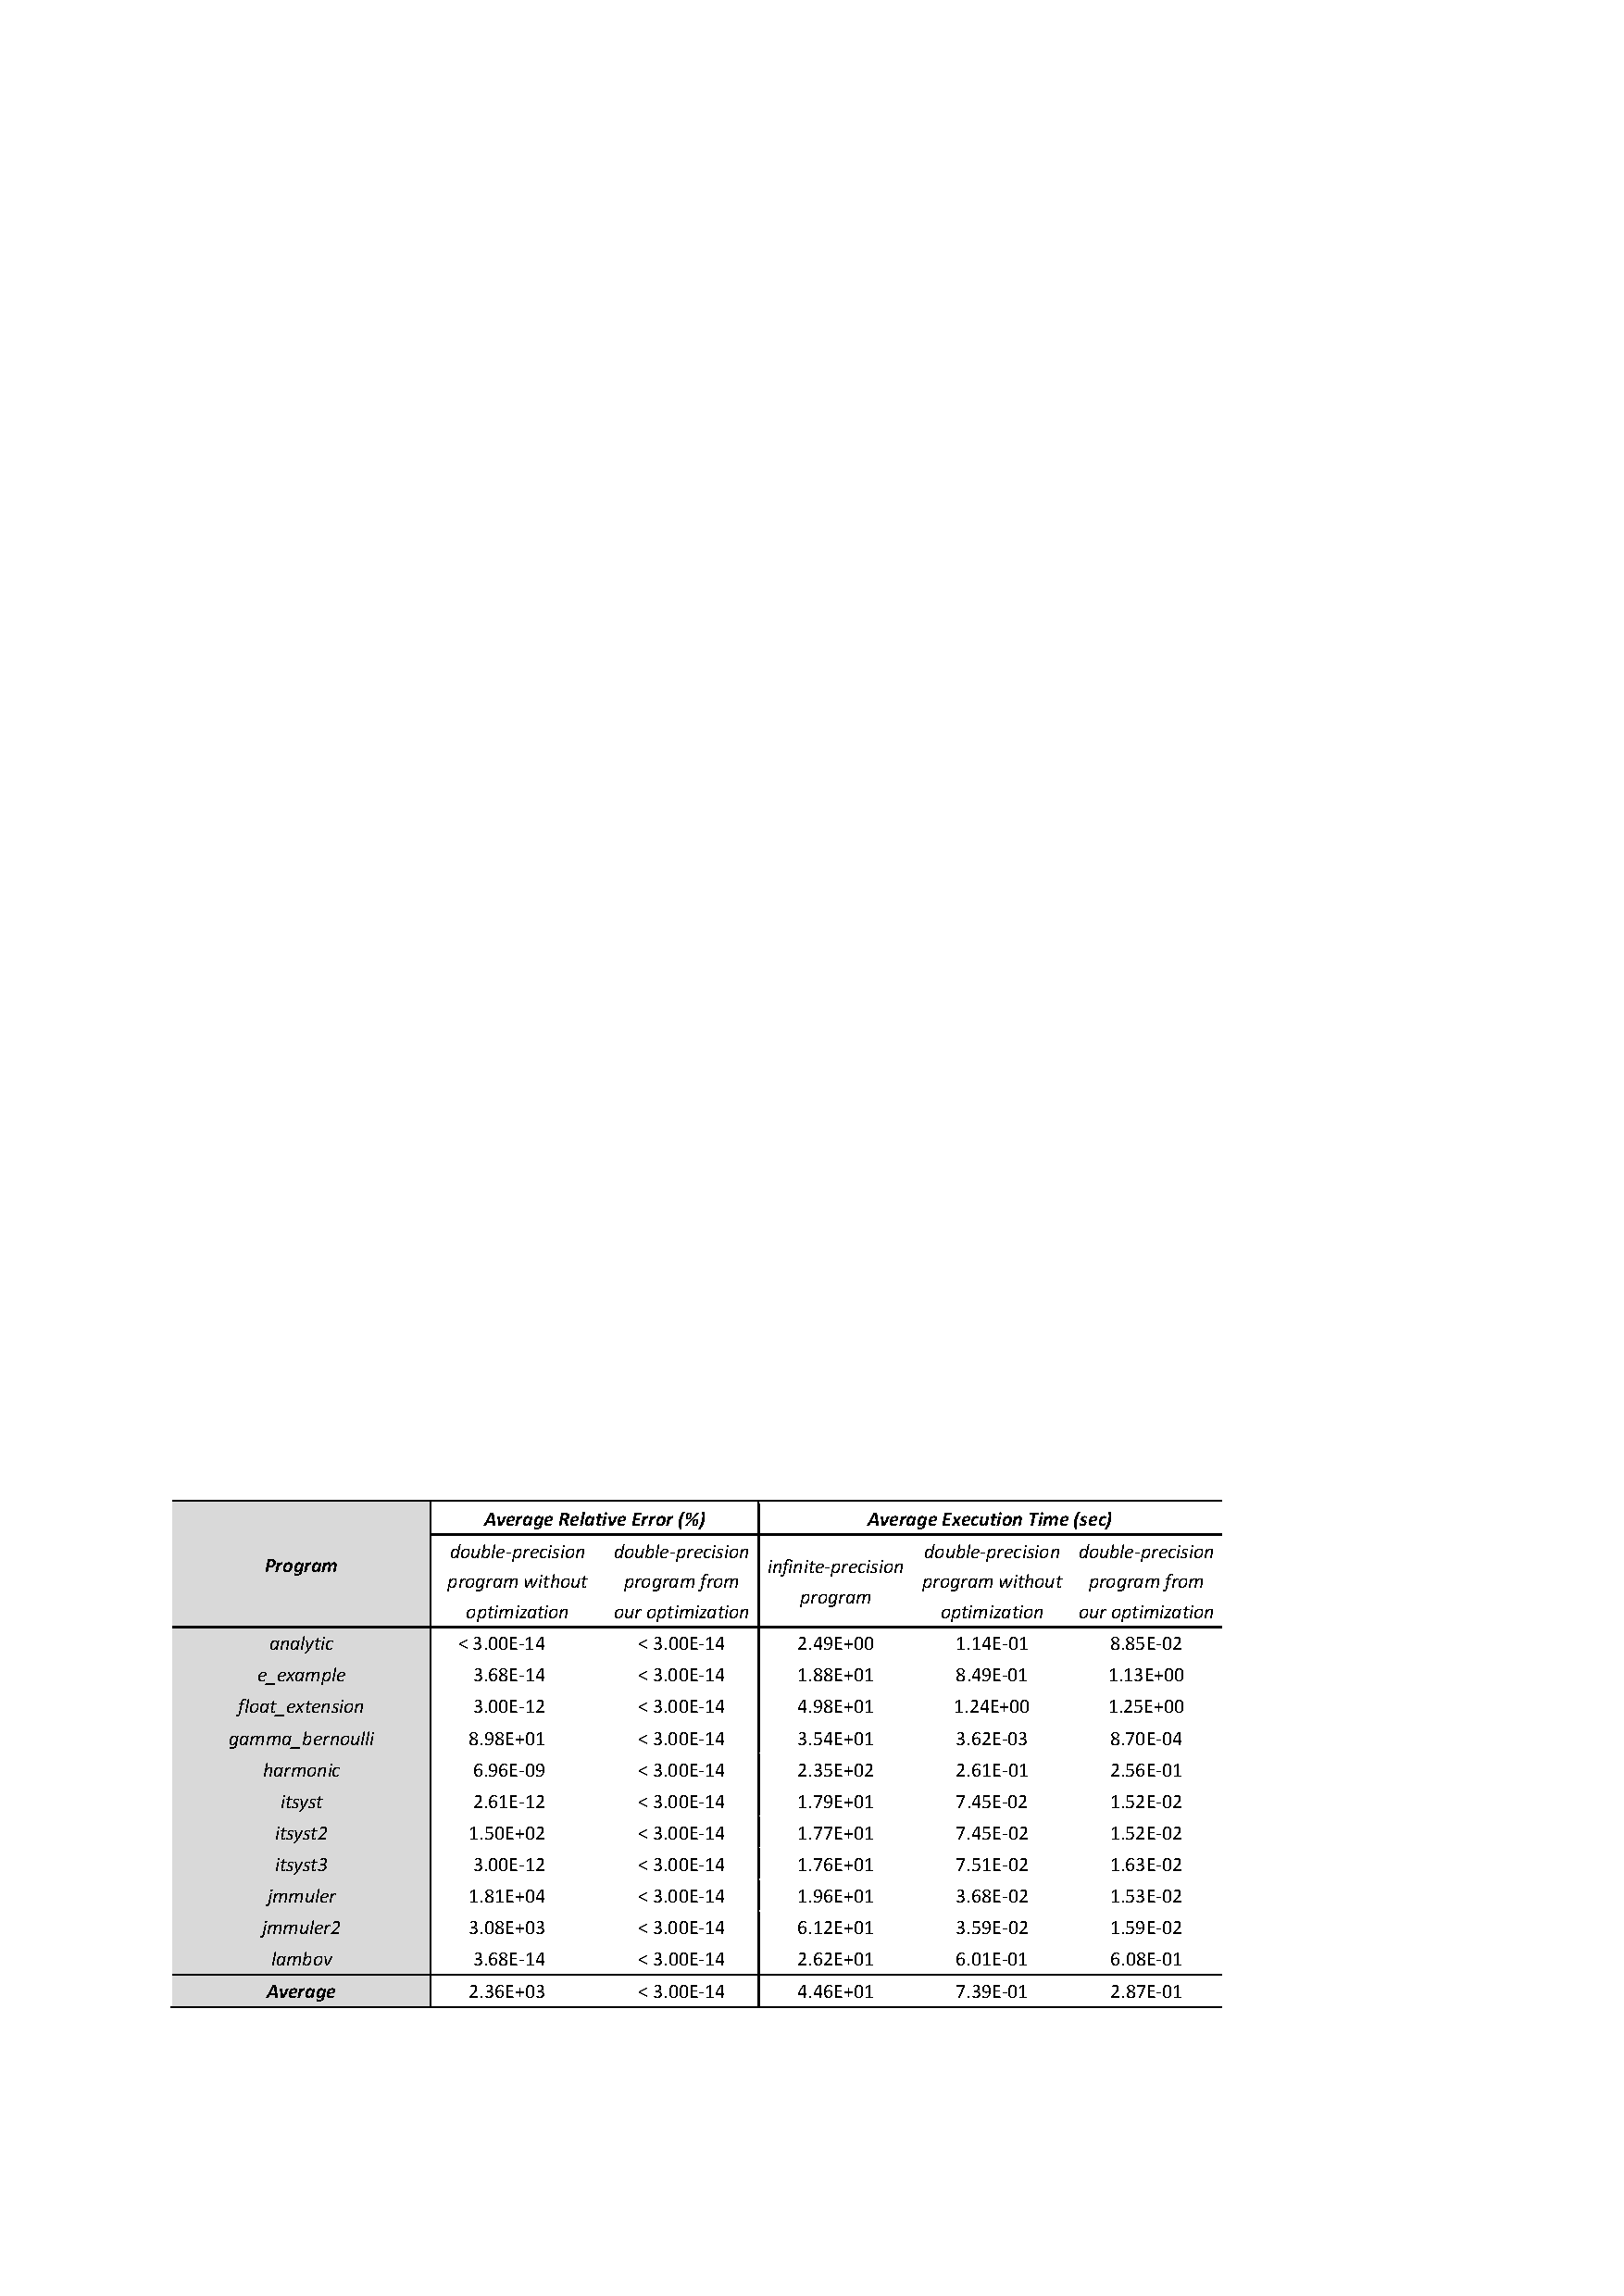
\includegraphics[width=\columnwidth]{fig/EvalTable_ErrorTime.pdf}
   \caption{iRRAM示例程序误差即运行时间表} \label{fig:error_time}
\end{table*}

\subsection{glibc数学函数库实验}

GNU C库是一个被广泛应用的C函数库,已有30年的历史,目前最主要的应用是配合Linux内核,是GNU/Linux操作系统的重要组成部分。在这个实验中,我们选取了GNU C库中部分常用的数据函数,使用任意精度对这些函数进行了重新实现,然后对这样的任意精度代码进行了优化,保证了优化后代码的正确性。然后,我们比较了这样重新实现的任意精度代码与原glibc中函数实现代码的一些可维护性指标,从而说明我们的优化工具能够帮助软件开发人员更加轻松地编写高可读性、可维护性并且正确高效的代码。

我们使用了业界常用的几种软件度量标准,包括了霍尔斯特德复杂度(Halstead Volume)、圈复杂度(Cyclomatic Complexity)以及可维护性指数(Maintainbility Index)。

霍尔斯特德复杂度是由霍尔斯特德在1977年提出的一种软件度量标准,其主要是依据程序源代码中的运算符和操作数来衡量源程序代码的复杂程度。在Halstead方法中,运算符是指用来处理程序中常量和变量的语法元素等,如算术运算符、逻辑运算符、关系运算符、流程控制语句、函数调用等;操作数则是指源程序代码中的常量和变量等,但对非执行语句,如注释,则不进行考虑。Halstead方法使用了以下4个基本测量数据:

\begin{itemize}
    \item 程序中运算符总数N1
    \item 程序中操作数总数N2
    \item 程序中运算符种类数n1
    \item 程序中操作数种类数n2
\end{itemize}

根据以上4个测量数据,可以在以下几个方面对源程序代码的复杂性进行度量:

\begin{itemize}
    \item 实际程序长度 N=N1+N2
    \item 编程语言层次 L=(2/n1)*(n2/N2)
    \item 程序容量 V=(N1+N2)*log2(n1+n2) 
    \item 预测程序长度 N'= n1*log2n1+n2*log2n2
    \item 估计程序工作量 E'=V/L=(n1*N2*(N1+N2)*log2(n1+n2))/(2*n2)
    \item 预测程序错误数E"=((N1+N2)*log2(n1+n2))/3000
\end{itemize}

在本次实验中,我们使用了程序容量V这一度量指标,这一指标代表了写一个程序所需的信息量,越高则表明该程序越难以开发和维护。

圈复杂度也被称作条件复杂度或是循环复杂度,是另一种代码复杂程度的衡量标准,是由 Thomas J. McCabezz,Sr. 在 1976 年提出,圈复杂度是对源代码中线性独立路径数的定量测量。

圈复杂度由程序的控制流图来计算,程序的控制流图是一个有向图,图中的节点为程序的基础模块,若一个模块结束后,可能会运行另一个模块,则用箭头链接二个模块,并标示可能的运行顺序。程序的圈复杂度由以下公式来计算:

\begin{align*}
    C = E - X + 2P
\end{align*}

其中 E 为图中边的个数, X 为图中节点的个数,P 为连接组件的个数。圈复杂度高说明程序代码的判断逻辑复杂,代码质量越低且更加难以测试和维护。

可维护性指数是一个结合了霍尔斯特德复杂度,圈复杂度以及代码行数的综合性指标,其计算公式如下所示:

\begin{align*}
    MI = 171 - 5.2\ln V - 0.23C - 16.2\ln LOC + 50\sin\sqrt{2.46CM}
\end{align*}

其中V代表了程序容量,C代表了程序圈复杂度,LOC代表了代码行数,CM代表了程序中的注释占总程序量的百分比,由于我们只考虑数学函数数值计算程序的具体代码实现,所以我们忽略计算公式中的CM。可维护性指数越低,表明程序越易于维护。

\begin{table*}[thbp]
    \centering
    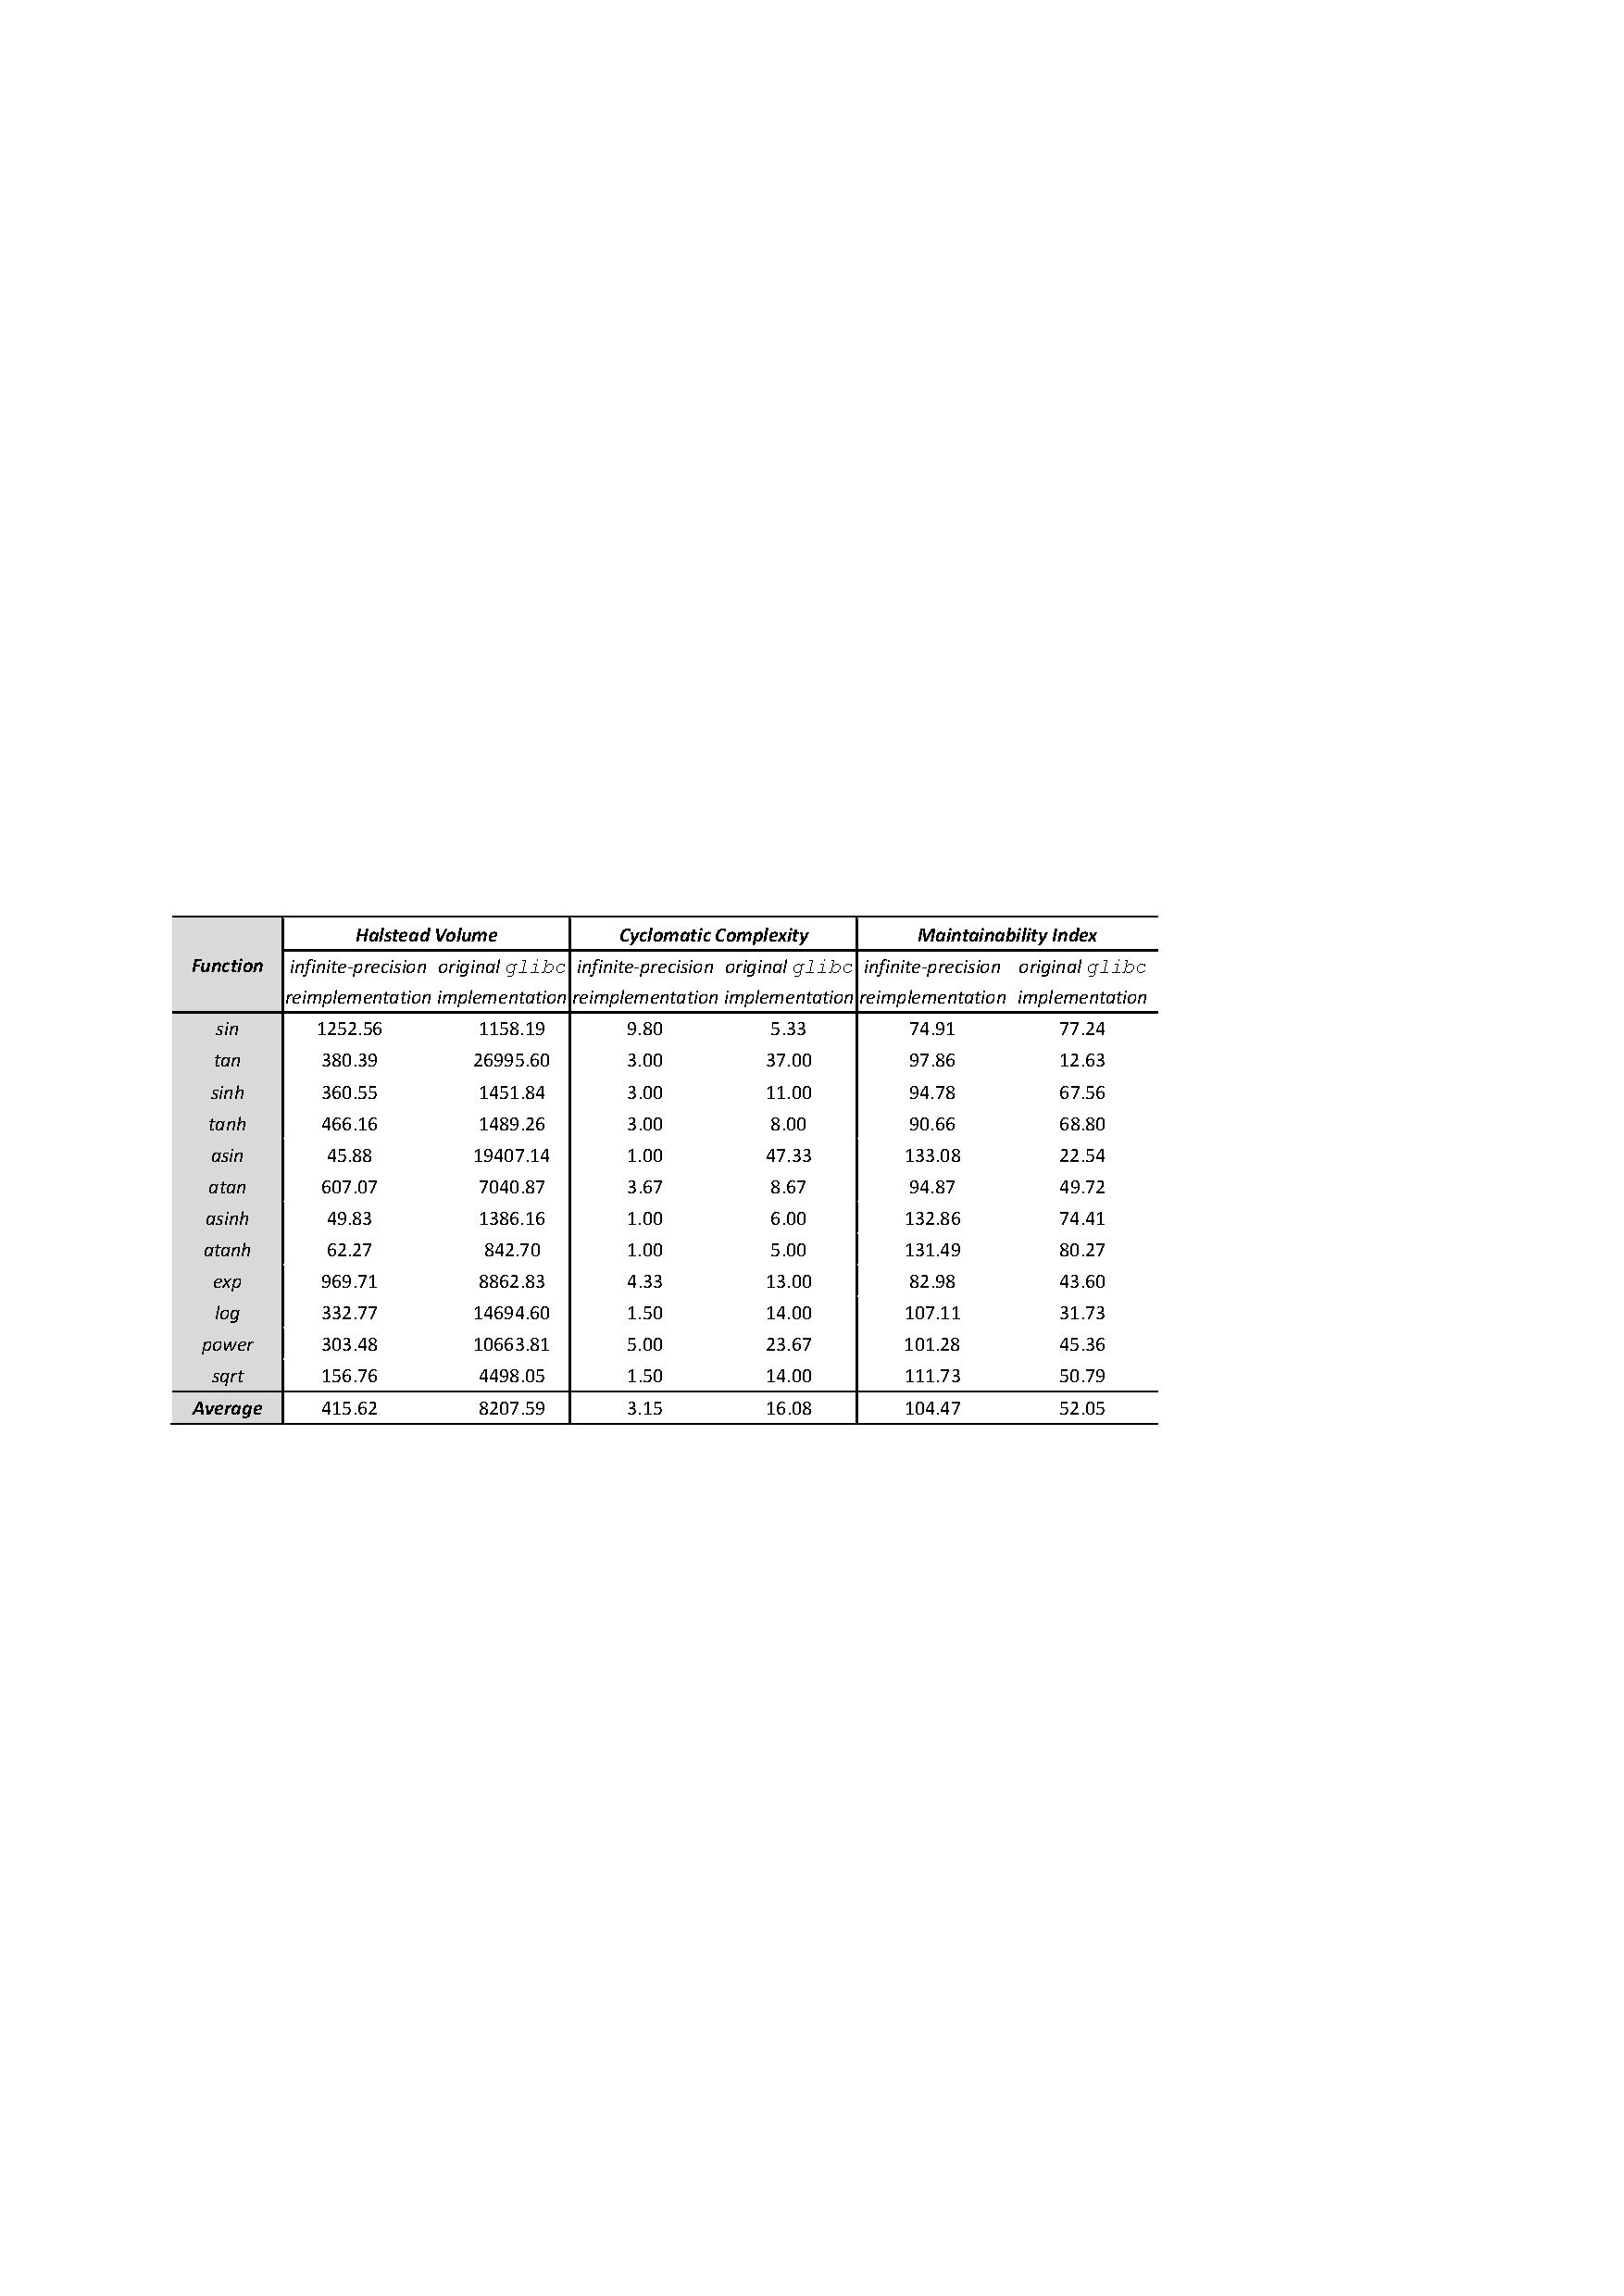
\includegraphics[width=\columnwidth]{fig/EvalTable_ComplexMeasurements.pdf}
    \caption{glibc数学函数在不同实现下各度量指标对比表} \label{fig:complex_measurements}
 \end{table*}

表\ref{fig:complex_measurements}展示了两种不同实现的个度量指标的对比,某些函数使用了大量相同的代码实现,其各项度量指标基本保持一致,因此我们在这里只列举了其中的一个(例如sin函数与cos函数)。从图中我们可以观察到,由于数值计算专家在实现浮点精度的数值计算程序时引入了大量的精度相关的操作,导致glibc的函数实现相比于我们使用任意精度实现的代码复杂了很多。任意精度代码的平均霍尔斯特德复杂度大概只有浮点精度代码的二十分之一,圈复杂度也仅仅只有任意精度代码的五分之一。浮点精度代码的平均可维护性指为104.47,是任意精度代码的两倍左右。从上述实验结果我们可以看出,使用任意精度编写代码,然后使用优化框架进行优化这样的开发数值计算程序的开发方式比直接使用浮点精度代码进行开发能够使程序更加简洁,具有更高的可读性与可维护性。于此同时,程序员即便不具备数值计算专家的专业知识,也能够开发出高效正确的数值计算代码。

\section{本章小结}

在本章中,我们基于上一章节中提到的数值程序的优化方法,实现了一个数值计算程序的优化工具NGOpt,并具体介绍了一些重点的模块,包括基于KLEE符号执行完成的路径提取模块,基于规则模板的随机代数变换引擎等。

随后我们进一步的说明了工具的使用方法,使用工具时各个配置项的具体含义。为了验证我们的工具在对于现实世界中的数值计算程序的优化效果,我们选取了iRRAM高精度数值计算库中的一系列测试程序进行了优化。结果表明,我们的工具能够在不影响程序正确性的情况下极大地提升数值计算程序的运行效率。而后,为了说明我们的工具能够帮助软件开发人员更加轻松地开发高效正确的数值计算代码,我们选取了gblic中部分常用的数学函数,比较了直接的浮点精度实现以及任意精度实现在各个度量指标上的表现,证明了我们的工具的确可以极大提升软件开发人员在开发数值计算程序时的开发效率,同时也能够使得数值计算程序更加易读易维护。

%%%%%%%%%%%%%%%%%%%%%%%%%%%%%%%%%%%%%%%%%%%%%%%%%%%%%%%%%%%%%%%%%%%%%%%%%%%%%%%
% 学位论文的正文应以《结论》作为最后一章
\chapter{结论}\label{chapter_concludes}

%%%%%%%%%%%%%%%%%%%%%%%%%%%%%%%%%%%%%%%%%%%%%%%%%%%%%%%%%%%%%%%%%%%%%%%%%%%%%%%
% 致谢,应放在《结论》之后
\begin{acknowledgement}
  首先感谢我的母亲韦春花对我的支持。其次感谢我的导师陈近南对我的精心指导和热心帮助。接下来,
  感谢我的师兄茅十八和风际中,他们阅读了我的论文草稿并提出了很有价值的修改建议。

  最后,感谢我亲爱的老婆们:双儿、苏荃、阿珂、沐剑屏、曾柔、建宁公主、方怡,感谢
  你们在生活上对我无微不至的关怀和照顾。我爱你们!
\end{acknowledgement}

%%%%%%%%%%%%%%%%%%%%%%%%%%%%%%%%%%%%%%%%%%%%%%%%%%%%%%%%%%%%%%%%%%%%%%%%%%%%%%%
% 附录
\appendix

\chapter{博士(硕士)学位论文编写格式规定(试行)}

\section{适用范围}

本规定适用于博士学位论文编写,硕士学位论文编写应参照执行。

\section{引用标准}

GB7713科学技术报告、学位论文和学术论文的编写格式。

GB7714文后参考文献著录规则。

\section{印制要求}

论文必须用白色纸印刷,并用A4(210mm×297mm)标准大小的白纸。纸的四周应留足空白
边缘,上方和左侧应空边25mm以上,下方和右侧应空边20mm以上。除前置部分外,其它
部分双面印刷。

论文装订不要用铁钉,以便长期存档和收藏。

论文封面与封底之间的中缝(书脊)必须有论文题目、作者和学校名。

\section{编写格式}

论文由前置部分、主体部分、附录部分(必要时)、结尾部分(必要时)组成。

前置部分包括封面,题名页,声明及说明,前言,摘要(中、英文),关键词,目次页,
插图和附表清单(必要时),符号、标志、缩略词、首字母缩写、单位、术语、名词解释
表(必要时)。

主体部分包括绪论(作为正文第一章)、正文、结论、致谢、参考文献表。

附录部分包括必要的各种附录。

结尾部分包括索引和封底。

\section{前置部分}

\subsection{封面(博士论文国图版用)}

封面是论文的外表面,提供应有的信息,并起保护作用。

封面上应包括下列内容:
\begin{enumerate}
\item 分类号  在左上角注明分类号,便于信息交换和处理。一般应注明《中国图书资
  料分类法》的类号,同时应注明《国际十进分类法UDC》的类号;
\item 密级  在右上角注明密级;
\item “博士学位论文”用大号字标明;
\item 题名和副题名   用大号字标明;
\item 作者姓名;
\item 学科专业名称;
\item 研究方向;
\item 导师姓名,职称;
\item 日期包括论文提交日期和答辩日期;
\item 学位授予单位。
\end{enumerate}

\subsection{题名}

题名是以最恰当、最简明的词语反映论文中最重要的特定内容的逻辑组合。

题名所用每一词语必须考虑到有助于选定关键词和编写题录、索引等二次文献可以提供
检索的特定实用信息。

题名应避免使用不常见的缩略词、首字母缩写字、字符、代号和公式等。

题名一般不宜超过20字。

论文应有外文题名,外文题名一般不宜超过10个实词。

可以有副题名。

题名在整本论文中不同地方出现时,应完全相同。

\subsection{前言}

前言是作者对本论文基本特征的简介,如论文背景、主旨、目的、意义等并简述本论文
的创新性成果。

\subsection{摘要}

摘要是论文内容不加注释和评论的简单陈述。

论文应有中、英文摘要,中、英文摘要内容应相同。

摘要应具有独立性和自含性,即不阅读论文的全文,便能获得必要的信息,摘要
中有数据、有结论,是一篇完整的短文,可以独立使用,可以引用,可以用于推广。摘
要的内容应包括与论文同等量的主要信息,供读者确定有无必要阅读全文,也供文摘等
二次文献引用。摘要的重点是成果和结论。

中文摘要一般在1500字,英文摘要不宜超过1500实词。

摘要中不用图、表、化学结构式、非公知公用的符号和术语。

\subsection{关键词}

关键词是为了文献标引工作从论文中选取出来用于表示全文主题内容信息款目的单词或
术语。

每篇论文选取3-8个词作为关键词,以显著的字符另起一行,排在摘要的左下方。在英
文摘要的左下方应标注与中文对应的英文关键词。

\subsection{目次页}

目次页由论文的章、节、附录等的序号、名称和页码组成,另页排在摘要的后面。

\subsection{插图和附表清单}

论文中如图表较多,可以分别列出清单并置于目次页之后。

图的清单应有序号、图题和页码。表的清单应有序号、表题和页码。

符号、标志、缩略词、首字母缩写、计量单位、名词、术语等的注释表符号、标志、缩略词、
首字母缩写、计量单位、名词、术语等的注释说明汇集表,应置于图表清单之后。

\section{主体部分}

\subsection{格式}

主体部分由绪论开始,以结论结束。主体部分必须由另页右页开始。每一章必须另页开
始。全部论文章、节、目的格式和版面安排要划一,层次清楚。

\subsection{序号}

\begin{figure}[htbp]
  \centering
  
\includegraphics[width= 0.5\textwidth]{njuname.eps}\\
  \caption{测试附录中的插图}\label{fig:appendix1}
\end{figure}

论文的章可以写成:第一章。节及节以下均用阿拉伯数字编排序号,如
1.1,1.1.1等。

论文中的图、表、附注、参考文献、公式、算式等一律用阿拉伯数字分别分章依序连续编排
序号。其标注形式应便于互相区别,一般用下例:图1.2;表2.3;附注1);文献[4];式
  (6.3)等。

论文一律用阿拉伯数字连续编页码。页码由首页开始,作为第1页,并为右页另页。封页、
封二、封三和封底不编入页码,应为题名页、前言、目次页等前置部分单独编排页码。页码
必须标注在每页的相同位置,便于识别。

\begin{equation}
    C_i = \frac{2E_i}{k_i(k_i-1)}
\end{equation}

附录依序用大写正体A、B、C、$\cdots$编序号,如:附录A。附录中的图、表、式、参考文
献等另行编序号,与正文分开,也一律用阿拉伯数字编码,但在数码前题以附条序码,如图
A.1;表B.2;式(B.3);文献[A.5]等。

\subsection{绪论}

绪论(综述):简要说明研究工作的目的、范围、相关领域的前人工作和知识空白、理
论基础和分析,研究设想、研究方法和实验设计、预期结果和意义等。一般在教科书中
有的知识,在绪论中不必赘述。

绪论的内容应包括论文研究方向相关领域的最新进展、对有关进展和问题的评价、本论
文研究的命题和技术路线等;绪论应表明博士生对研究方向相关的学科领域有系统深入
的了解,论文具有先进性和前沿性;

\begin{problem}
测试定理环境。测试定理环境。测试定理环境。测试定理环境。测试定理环境。测试定理环境。
测试定理环境。测试定理环境。测试定理环境。
\end{problem}

为了反映出作者确已掌握了坚实的基础理论和系统的专门知识,具有开阔的科学视野,对研
究方案作了充分论证,绪论应单独成章,列为第一章,绪论的篇幅应达$1\sim 2$万字,不
得少于$1$万字;绪论引用的文献应在$100$篇以上,其中外文文献不少于$60\%$;引用文献
应按正文中引用的先后排列。

\subsection{正文}

论文的正文是核心部分,占主要篇幅。正文必须实事求是,客观真切,准确完备,合乎
逻辑,层次分明,简便可读。

\begin{figure}[htbp]
  \centering
  
\includegraphics[width= 0.5\textwidth]{njuname.eps}\\
  \caption{测试附录中的插图}\label{fig:appendix2}
\end{figure}

正文的每一章(除绪论外)应有小结,在小结中应明确阐明作者在本章中所做的工作,特
别是创新性成果。凡本论文要用的基础性内容或他人的成果不应单独成章,也不应作过
多的阐述,一般只引结论、使用条件等,不作推导。

\subsubsection{图}

图包括曲线图、构造图、示意图、图解、框图、流程图、记录图、布置图、地图、照片
、图版等。

图应具有“自明性”,即只看图、图题和图例,不阅读正文,就可以理解图意。

图应编排序号。每一图应有简短确切的图题,连同图号置于图下。必要时,应将图上的
符号、标记、代码,以及实验条件等,用最简练的文字,横排于图题下方,作为图例说
明。

\begin{example}
测试定理环境。测试定理环境。测试定理环境。测试定理环境。测试定理环境。测试定理环境。
测试定理环境。测试定理环境。测试定理环境。
\end{example}

曲线图的纵、横坐标必须标注“量、标准规定符号、单位”。此三者只有在不必要标明
(如无量纲等)的情况下方可省略。坐标上标注的量的符号和缩略词必须与正文一致。

照片图要求主题和主要显示部分的轮廓鲜明,便于制版。如用放大缩小的复制品,必须
清晰,反差适中。照片上应该有表示目的物尺寸的标度。

\subsubsection{表}

表的编排,一般是内容和测试项目由左至右横读,数据依序竖排。表应有自明性。

表应编排序号。

每一表应有简短确切的表题,连同标号置于表上。必要时,应将表中的符号、标记、代
码,以及需要说明事项,以最简练的文字,横排于表题下,作为表注,也可以附注于表
下。表内附注的序号宜用小号阿拉伯数字并加圆括号置于被标注对象的右上角,如:
xxx${}^{1)}$;不宜用“*”,以免与数学上共轭和物质转移的符号相混。

表的各栏均应标明“量或测试项目、标准规定符号、单位”。只有在无必要标注的情况下
方可省略。表中的缩略词和符号,必须与正文中一致。

表内同一栏的数字必须上下对齐。表内不宜用“同上”,“同左”和类似词,一律填入具体数字
或文字。表内“空白”代表未测或无此项,“-”或“\textellipsis”(因“-”可能与代表阴性
  反应相混)代表未发现,“0”代表实测结果确为零。

如数据已绘成曲线图,可不再列表。

\subsubsection{数学、物理和化学式}

正文中的公式、算式或方程式等应编排序号,序号标注于该式所在行(当有续行时,应
标注于最后一行)的最右边。

较长的式,另行居中横排。如式必须转行时,只能在$+$,$-$,$\times$,$\div$,$<$,
$>$处转行。上下式尽可能在等号“$=$”处对齐。

小数点用“$.$”表示。大于$999$的整数和多于三位数的小数,一律用半个阿拉伯数字符的小
间隔分开,不用千位撇。对于纯小数应将$0$列于小数点之前。

示例:应该写成$94\ 652.023\ 567$和$0.314\ 325$, 不应写成$94,652.023,567$和
$.314,325$。

应注意区别各种字符,如:拉丁文、希腊文、俄文、德文花体、草体;罗马数字和阿拉伯数
字;字符的正斜体、黑白体、大小写、上下脚标(特别是多层次,如“三踏步”)、上下偏差
等。

\subsubsection{计量单位}

报告、论文必须采用国务院发布的《中华人民共和国法定计量单位》,并遵照《中华人
民共和国法定计量单位使用方法》执行。使用各种量、单位和符号,必须遵循附录B所
列国家标准的规定执行。单位名称和符号的书写方式一律采用国际通用符号。

\subsubsection{符号和缩略词}

符号和缩略词应遵照国家标准的有关规定执行。如无标准可循,可采纳本学科或本专业
的权威性机构或学术团体所公布的规定;也可以采用全国自然科学名词审定委员会编印
的各学科词汇的用词。如不得不引用某些不是公知公用的、且又不易为同行读者所理解
的、或系作者自定的符号、记号、缩略词、首字母缩写字等时,均应在第一次出现时一
一加以说明,给以明确的定义。

\subsection{结论}

报告、论文的结论是最终的、总体的结论,不是正文中各段的小结的简单重复。结论应
该准确、完整、明确、精炼。在结论中要清楚地阐明论文中有那些自己完成的成果,特
别是创新性成果;

如果不可能导出应有的结论,也可以没有结论而进行必要的讨论。可以在结论或讨论中
提出建议、研究设想、仪器设备改进意见、尚待解决的问题等。

\subsection{致谢}

可以在正文后对下列方面致谢:

\begin{itemize}
\item 国家科学基金、资助研究工作的奖学金基金、合作单位、资助或支持的企业、组织或个
人;
\item 协助完成研究工作和提供便利条件的组织或个人;
\item 在研究工作中提出建议和提供帮助的人;
\item 给予转载和引用权的资料、图片、文献、研究思想和设想的所有者;
\item 其他应感谢的组织或个人。
\end{itemize}

\subsection{参考文献表}

\subsubsection{专著著录格式}

主要责任者,其他责任者,书名,版本,出版地:出版者,出版年

例:1. 刘少奇,论共产党员的修养,修订2版,北京:人民出版社,1962

\subsubsection{连续出版物中析出的文献著录格式}

析出文献责任者,析出文献其他责任者,析出题名,原文献题名,版本:文献中的位置。

例:2. 李四光,地壳构造与地壳运动,中国科学,1973 (4):400-429

参考文献采用顺序编码制,按论文正文所引用文献出现的先后顺序连续编码。

\section{附录}

附录是作为报告、论文主体的补充项目,并不是必需的。

下列内容可以作为附录编于报告、论文后,也可以另编成册;

\begin{enumerate}
\item 为了整篇论文材料的完整,但编入正文又有损于编排的条理和逻辑性,这一材料
包括比正文更为详尽的信息、研究方法和技术更深入的叙述,建议可以阅读的参考文献
题录,对了解正文内容有用的补充信息等;
\item 由于篇幅过大或取材于复制品而不便于编入正文的材料;
\item 不便于编入正文的罕见珍贵资料;
\item 对一般读者并非必要阅读,但对本专业同行有参考价值的资料;
\item 某些重要的原始数据、数学推导、计算程序、框图、结构图、注释、统计表、计
算机打印输出件等。
\end{enumerate}

附录与正文连续编页码。

每一附录均另页起。

\section{结尾部分 (必要时)}

为了将论文迅速存储入电子计算机,可以提供有关的输入数据。可以编排分类索引、著者索
引、关键词索引等。

% 参考文献。应放在\backmatter之前。
% 推荐使用BibTeX,若不使用BibTeX时注释掉下面一句。
\nocite{*}
\bibliography{sample}
% 不使用 BibTeX
%\begin{thebibliography}{2}
%
%\bibitem{deng:01a}
%{邓建松,彭冉冉,陈长松}.
%\newblock {\em \LaTeXe{}科技排版指南}.
%\newblock 科学出版社,书号:7-03-009239-2/TP.1516, 北京, 2001.
%
%\bibitem{wang:00a}
%王磊.
%\newblock {\em \LaTeXe{}插图指南}.
%\newblock 2000.
%\end{thebibliography}

% 附录,必须放在参考文献后,backmatter前
\appendix
\chapter{图论基础知识}
\Blindtext

%%%%%%%%%%%%%%%%%%%%%%%%%%%%%%%%%%%%%%%%%%%%%%%%%%%%%%%%%%%%%%%%%%%%%%%%%%%%%%%
% 书籍附件
\backmatter
%%%%%%%%%%%%%%%%%%%%%%%%%%%%%%%%%%%%%%%%%%%%%%%%%%%%%%%%%%%%%%%%%%%%%%%%%%%%%%%
% 作者简历与科研成果页,应放在backmatter之后
\begin{resume}
% 论文作者身份简介,一句话即可。
\begin{authorinfo}
\noindent 韦小宝,男,汉族,1985年11月出生,江苏省扬州人。
\end{authorinfo}
% 论文作者教育经历列表,按日期从近到远排列,不包括将要申请的学位。
\begin{education}
\item[2007年9月 --- 2010年6月] 南京大学计算机科学与技术系 \hfill 硕士
\item[2003年9月 --- 2007年6月] 南京大学计算机科学与技术系 \hfill 本科
\end{education}
% 论文作者在攻读学位期间所发表的文章的列表,按发表日期从近到远排列。
\begin{publications}
\item Xiaobao Wei, Jinnan Chen, ``Voting-on-Grid Clustering for Secure
  Localization in Wireless Sensor Networks,'' in \textsl{Proc. IEEE International
    Conference on Communications (ICC) 2010}, May. 2010.
\item Xiaobao Wei, Shiba Mao, Jinnan Chen, ``Protecting Source Location Privacy
  in Wireless Sensor Networks with Data Aggregation,'' in \textsl{Proc. 6th
    International Conference on Ubiquitous Intelligence and Computing (UIC)
    2009}, Oct. 2009.
\end{publications}
% 论文作者在攻读学位期间参与的科研课题的列表,按照日期从近到远排列。
\begin{projects}
\item 国家自然科学基金面上项目``无线传感器网络在知识获取过程中的若干安全问题研究''
(课题年限~2010年1月 --- 2012年12月),负责位置相关安全问题的研究。
\item 江苏省知识创新工程重要方向项目下属课题``下一代移动通信安全机制研究''
(课题年限~2010年1月 --- 2010年12月),负责LTE/SAE认证相关的安全问题研究。
\end{projects}
\end{resume}

%%%%%%%%%%%%%%%%%%%%%%%%%%%%%%%%%%%%%%%%%%%%%%%%%%%%%%%%%%%%%%%%%%%%%%%%%%%%%%%
% 生成《学位论文出版授权书》页面,应放在最后一页
\makelicense

%%%%%%%%%%%%%%%%%%%%%%%%%%%%%%%%%%%%%%%%%%%%%%%%%%%%%%%%%%%%%%%%%%%%%%%%%%%%%%%
\end{document}
